\chapter{Electrophysiology of the Heart}


The heart functions as a pump supplying rich-oxygen blood to every part of the
body. Depending on the body's demand, it can squeeze fast or slow.
The electrical signal propagation inside the heart is described as follows.
Excitation of the heart is {\bf myogenic}, i.e. contraction of the heart
originates within the muscle itself. The cells that are most leaky to calcium
initiate action potentials more frequently and set the rate of contraction for
entire heart structure. \textcolor{red}{Each region of the heart has its own
intrinsic rate of beating}.  For example, in mammals, the SA node (embedded in
the wall of the atrium) = 72 b/min, atrium = 60 b/min, ventricle 25 b/min.  Only
when faster  beating chambers are electrochemically separated from the slower
can the  intrinsic beat rate of the slower chambers be seen.   
The frequency of depolarization of the sinus venosus is modified by inputs from
the {\it autonomic nervous system}. Autonomic nervous system is a component of
the motor component of the {\it peripheral nervous system}.  


Fig.\ref{fig:signal2heart} describes how the heart receives the electrical
signal from different parts of the body. Baroreceptors is a mechanoreceptor that
detects the pressure of blood flowing through them, and send the signal to the
central nervous system (CNS) to adjust (increase/decrease) total peripheral
resistance or cardiac output. It responses quickly, but the response diminish
with time, so its main function is to convey short term changes in blood
pressure. When there's a sustained increase of blood pressure for long time,
other receptors will take over the regulation. 

\section{From the brain to the heart}
\label{sec:brain-to-heart-connection}

Information passing from the central nervous system to a target organ must pass
through two neurons - one with its cell body within the {\it spinal cord}
(Sect.\ref{sec:spinal_cord}) and one with its cell body in a {\it ganglion}
located peripheral to the CNS.

Sympathetic ganglia are mostly located close to the spinal cord in the
sympathetic ganglion or chain ganglion, located parallel to the spinal cord.
Parasympathetic ganglia are mostly located directly adjacent to their target
organ in what are collectively called peripheral ganglia or terminal ganglia.

\section{Heart rate - sympathetic control}
\label{sec:sympathetic_control-heart-rate}
\label{sec:heart-rate}

In human, averate heart rate (at rest) is 70bpm for normal adults, and higher
for children. During sleep, in human, the heart rate reduce by 10-20 bpm.
For a well-trained atheletes, the resting heart rate is slower, e.g. 50 bpm.

Among the many factors that can control the heart rate (e.g.
temperature, stretching of the tissue), the sympathetic nervous system
(Sect.\ref{sec:sympathetic_nervous system}) of the {\it autonomous nervous
system} (ANS) is the dominant one (Sect.\ref{sec:autonomic_nervous_system}), at
T1-T4 segments of the thoracic nerves Fig.\ref{fig:sympathetic_nerve_cardiac}.
Impairment of the CNS, mostly in patients with high thoracic spinal cord injury
(SCI), can cause cardiac arrhythmias (esp. bradycardia). Annual incidence of SCI
is 15-52.5 cases per 1 mil. population \citep{grigorean2009}.

\begin{figure}[hbt]
  \centerline{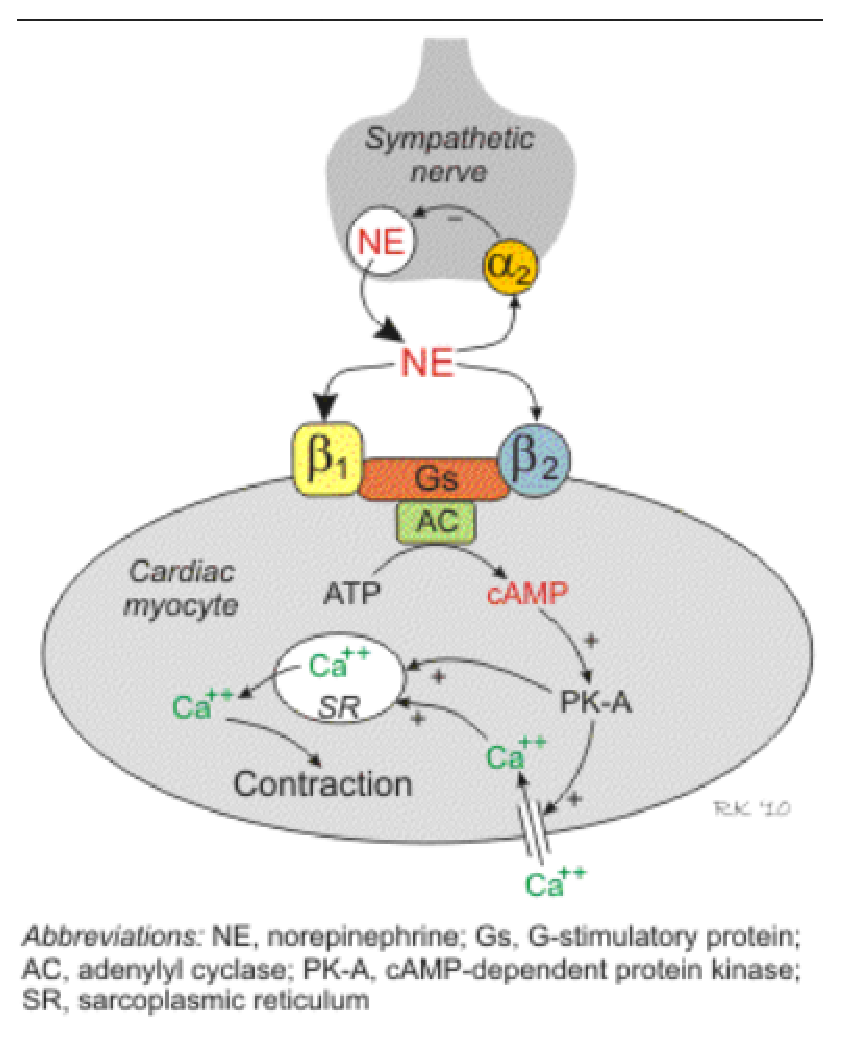
\includegraphics[height=9cm,
    angle=0]{./images/sympathetic_nerve_cardiac.eps}}
  \caption{How sympathetic nerve control heart rate
  \url{http://www.cvpharmacology.com/cardiostimulatory/beta-agonist.htm}}
  \label{fig:sympathetic_nerve_cardiac}
\end{figure}

The control of heart rates by ANS was investigated by \citep{Robinson1966}. He
has three group: (1) blocking cardiac sympathetic nerves, (2) blocking
parasympathetic nerve, and (3) both.
\begin{enumerate}
  \item block cardiac sympathetic nerve (which is similar to blocking
  $\beta$-receptors): can be done using $\beta$-adrenergic blocker like
  propranolol (dose: 0.25mg/kg. NOTE: 0.15mg/kg induces the  effectiveness of
  infused isoproterenol (ISO) at least 90\%).
  
NOTE: \textcolor{red}{In cell experiments: $\beta$-adrenergic stimulus can be
used to mimic the effect of cardiac sympathetic nerve}
(Sect.\ref{sec:beta-adrenergic_stimulation}).

  \item block parasympathetic nerve: can be done using 2 mg of atrophine given
  intravenously (i.e. giving fluid directly into the vein)
\end{enumerate}



\subsection{Sympathetic stimulation}
\label{sec:sympathetic-stimulation}

{\bf Sympathetic stimulation} (Sect.\ref{sec:sympathetic_nervous system}) speeds
up the sinus node ({\it sinus tachycardia}), while vagal activity
(parasympathetic input from the vagus nerve - cranial nerve X -
Sect.\ref{sec:cranial-nerve}) slows the node ({\it sinus bradycardia}).

The neurotransmitter used at both synapses in the parasympathetic route is
acetylcholine (ACh - Sect.\ref{sec:Acetylcholine}) which slows down the
intrinsic rate of the cardiac muscle contraction by activating muscarinic
receptors and vagal stimulation.

\textcolor{red}{Acetylcholine is the first neurotransmitter in the sympathetic
system; and norepiphrine (NE; also called noradrenaline) is the second
neurotransmitter of the sympathetic route} (Sect.\ref{sec:norepinephrine}.
\begin{itemize}
  \item {\bf Norepiphrine} is increased in response to fear (by activating
$\alpha$-adrenergic constrictor receptors), while adrenaline is increased in
response to metabolic or global challenges in homeostasis (by activating
$\beta$-adrenergic vasodilator receptors).

  \item  {\bf Epinephrine} (EPI; also called adrenaline) released by the adrenal
 medulla reaches the same synapses via the blood and has the equivalent effect.
\end{itemize}

The increased contractility of ventricle ({\it positive inotropic state}),
increased frequency ({\it positive chronotropic state}), increased conduction
velocity ({\it positive bathmotropic state}) is triggered by noradrenaline (aka
norepiphrine, a main neurotransmsitter of sympathetic nerves) or adrenaline (a
main hormone secreted from adrenal glands).


\begin{figure}[hbt]
 \centerline{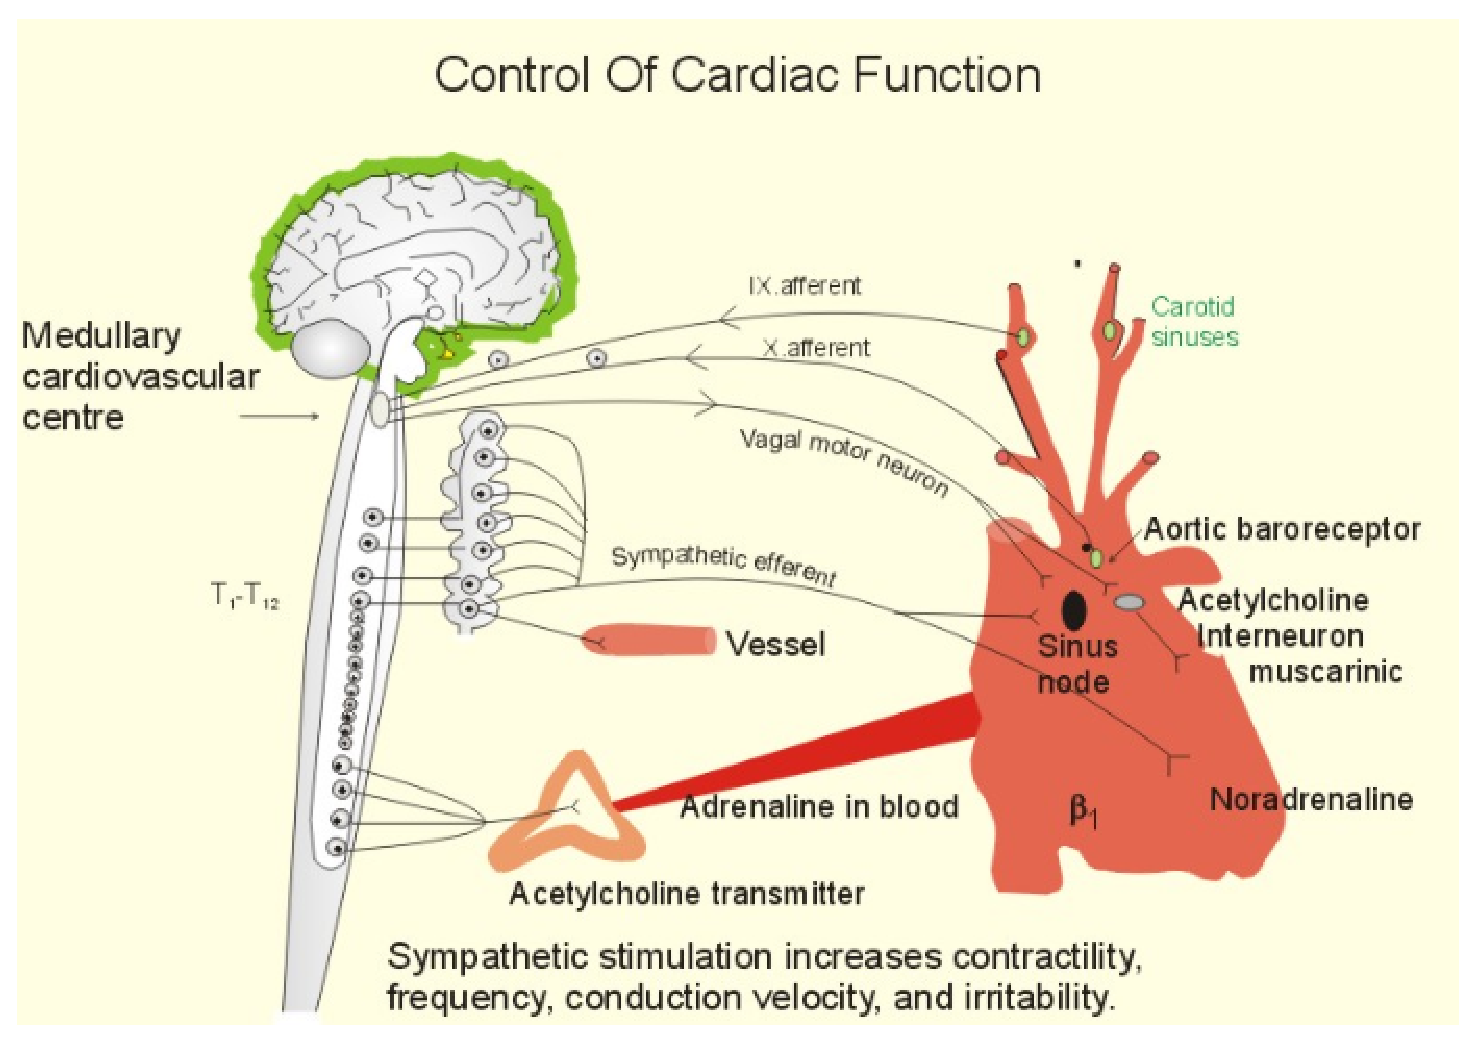
\includegraphics[height=7cm]{./images/signal2heart.eps}}
 \caption{\url{http://www.zuniv.net/physiology/book/images/11-1.jpg}}
\label{fig:signal2heart}
\end{figure}

\subsection{Parasympathetic input}



\section{Re-entry}
\label{sec:re-entry}


\url{https://en.wikipedia.org/wiki/Cardiac_arrhythmia#Re-entry}


\section{Effects of catecholamines on adrenergic receptors}

The heart have both $\beta_1$-AR and $\beta_2$-AR
(Sect.\ref{sec:beta-adrenergic-receptor}), and some species with $\beta_3$, yet
$\beta_1$-AR is the dominant one. $\beta_1$-AR coupled to Gs is the main one
responsible for inotropic effects and chronotropic effects of catecholamines
(Sect.\ref{sec:Catecholamines}).
\citep{Buxton1985} showed that in rat ventricles, only $\beta_1$-AR is found.

\begin{framed}
chronotropic effect = change heart rate

inotropic effect = change contraction force

dromotropic effect = agent that change the conduction speed in the AV node,
which subsequently affect the rate of electrical impulses in the heart. So,
agents that are dromotropic, are often (but not always) chronotropic and
inotropic.
\end{framed}

Under $\beta$-AR stimulation, $\beta$-AR preferentially coupled with Gs protein,
which in turns activate the enzyme {\it adenylyl cyclase} (AC)
(Sect.\ref{sec:AC_adenylyl_cyclase}). All classes of AC catalyze the conversion
of ATP to cAMP (Sect.\ref{sec:cAMP}) production [NOTE: This process requires
$\Mg$].

$\alpha_1$-AR (Sect.\ref{sec:adrenergic_receptor}) coupled to Gq cause an
increase $[\Ca]_i$ leading to smooth muscle contraction.
$\alpha_2$-AR also found in pre-synaptic in nerve cells, thus called {\it
presynaptic $\alpha_2$}-AR whose activation by NE inhibits the release of its
own NE hormone. $\alpha_1$-AR is found predominantly in vascular smooth muscle.

\citep{Landzberg1991} didn't found any role of $\alpha$-AR in maintaining basal
left ventricular contractile state in human, yet it has positive inotropic
effect (i.e. increasing heart rate)\footnote{a drug with inotropic effect is the
one that change force of contraction} whose magnitude can be attenuated (weaken)
in patients with heart failures. Reviews of $\alpha$-AR in heart failure:
\citep{shannon2006}.

In normal heart, the dominant beta-AR is $\beta_1$; while $\beta_2$-AR is the
dominant one in vascular and non-vascular smooth muscles. Activation of
$\beta_1$-AR leads to the increase in contractile force and heart rate; yet
activation of $\beta_2$-AR induces relaxation in vascular and non-vascular
smooth muscle. 

In patients with heart failures, applying drugs acting on $\beta_1$-AR though
increase the heart rates, excess stimulation can induce arrhythmias. Drugs
acting on $\beta_2$-AR can be used to treat as asthma (by relaxing airway smooth
muscle) and premature labor (by relaxing uterine smooth muscle).




Effects of different drugs is given in Fig.\ref{fig:heart_rate_drugs}. Atrophine
is an muscarinic receptors antagonist that blocks the parasympathetic effects,
so increasing the heart rates. Propranolol is a $\beta$-adrenergic receptor
antagonist that block sympathetic effects, i.e. decreasing the heart rate
\footnote{\url{https://www.inkling.com/read/berne-and-levy-physiology-updated-koeppen-stanton-6th/chapter-18/nervous-control-of-the-heart}}.

\begin{figure}[hbtp]
  \centerline{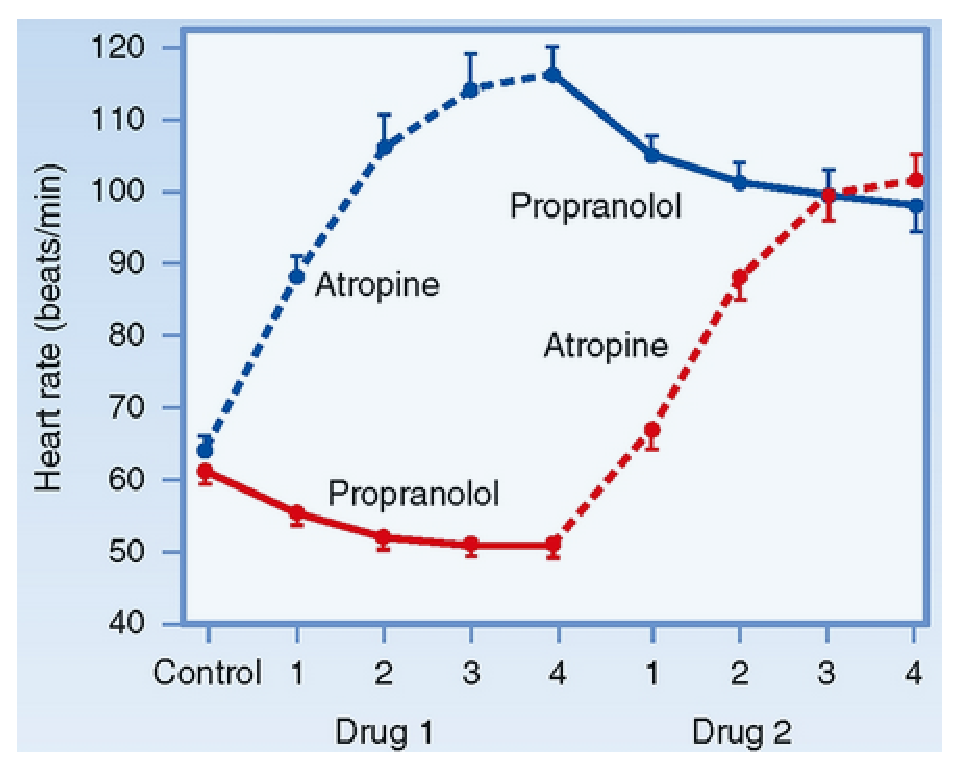
\includegraphics[height=7cm,
    angle=0]{./images/heart_rate_drugs.eps}}
  \caption{Effect of drugs (same dose) on the heart rates}
  \label{fig:heart_rate_drugs}
\end{figure}

The result of \citep{Robinson1966} showed that in mild exercise, cardiac
acceleration (heart rate) is controlled dominantly by decrease in
parasympathetic stimulus; while in heavy exercise, the effect of sympathetic
stimulation become more apparent. However, during tilting (e.g. 80$^\circ$
head-up tilt), sympathetic stimulus plays a dominant role than parasympathetic
stimulus, i.e. increasing heart rate. This was explained by the change in
arterial pressure between exercise and tilting.


\subsection{\texorpdfstring{$\beta$-adrenergic stimulation}{beta-adrenergic
stimulation}}
\label{sec:beta-adrenergic_stimulation}

$\beta$-adrenergic receptors (or rhodopsin) engage their signalling cascade by
collision coupling. With collision coupling, all receptors have unrestricted
access to all G proteins. In restricted collision coupling (which is the case
for A2A receptor - Sect.\ref{sec:A2A-receptor-binding}), the receptor is
allocated its particular lot of G proteins, there are no spare receptors.
In collision coupling, the concentration-response curve for agonists is shifted
to the left. Changes in receptor number, therefore, translate in changes of the
maximum response Emax rather than in EC50 values.

$\beta$-adrenergic receptor ($\beta$-AR) stimulation is used to mimic the effect
of sympathetic control of the ANS (Sect.\ref{sec:autonomic_nervous_system})in
the heart (Sect.\ref{sec:sympathetic_control-heart-rate}). $\beta$-AR
stimulation in the heart results in a significant increase in LCC (which leads
to increase RyR $\Ca$ flux via CICR mechanism).

There are 3 types of $\beta$-adrenergic receptors
(Sect.\ref{sec:beta-adrenergic-receptor}).
The underlying molecular mechanism is that the above channels (LCC, RyR) are
phosphorylated by the cAMP/PKA pathway (Sect.\ref{sec:cAMP-dependent_pathway})
\citep{Kamp2000, Reiken2003, hain1994}. Effect of $\beta$-adrenergic stimulation
in computational models was studied by \citep{koh2006}.


\section{Rate-dependent prolong APD}

Unlike most species, where the high pacing frequency reduce the APD, in rat
ventricular myocyte, the high physiological rate (1-5.7Hz) prolongs APD.

At high pacing rate, facilitation occurs in $I_\CaL$. Facilitation means that
the channel's inactivation is reduced, which bring the peak higher and the decay
is slower (Sect.\ref{sec:facilitation_CaMKII}). It has been showed that facilitation is not
observed when using depolarized holding potentials or prepulse \citep{brette2006cc}.


\section{Rate-dependent shortening APD}

A basic heart-cycle start with an APD, then a diastolic interval (DI), before
another APD starts. An important feature in the normal functioning of the heart
is APD change with the heart rate (i.e. DI is changed). In particular, APD is
shorten with an increase in heart rate, Fig.\ref{fig:APD_restitution} \citep{boyett1978}.

\begin{enumerate}
  
  \item In the intact heart: this is due to the action of adrenaline (i.e.
  targeting to adrenergic receptors) \citep{morad1972}. NOTE: There are
  two types: $\alpha$ or $\beta$ adrenalic receptor (adrenaline/noradrenaline),
  each has several subtypes ($\alpha_1, \alpha_2, \beta_1, \beta_2, \beta_3$).
  \textcolor{red}{In heart, we focus on $\beta_1$-type} (increase cardiac
  output). Agonists binding to $\beta$-adrenergic receptors cause a rise in
  cyclic-AMP (cAMP), a second messenger whose downstream effectors include
  cAMP-dependent  protein kinase (PKA). This is  important as PKA mediates many
  important  intracellular events. 
  
  \item In isolated cardiac myocyte: not from adrenaline, but something else ??? 
  \textcolor{red}{The APD depends on the processes responsible for the
  repolarization of the cell membrane}. 
\end{enumerate}
 
\subsection{In tissue}

The spatial dispersion of repolarization could be the result from the
differences in APD.

\begin{figure}[hbt]
 \centerline{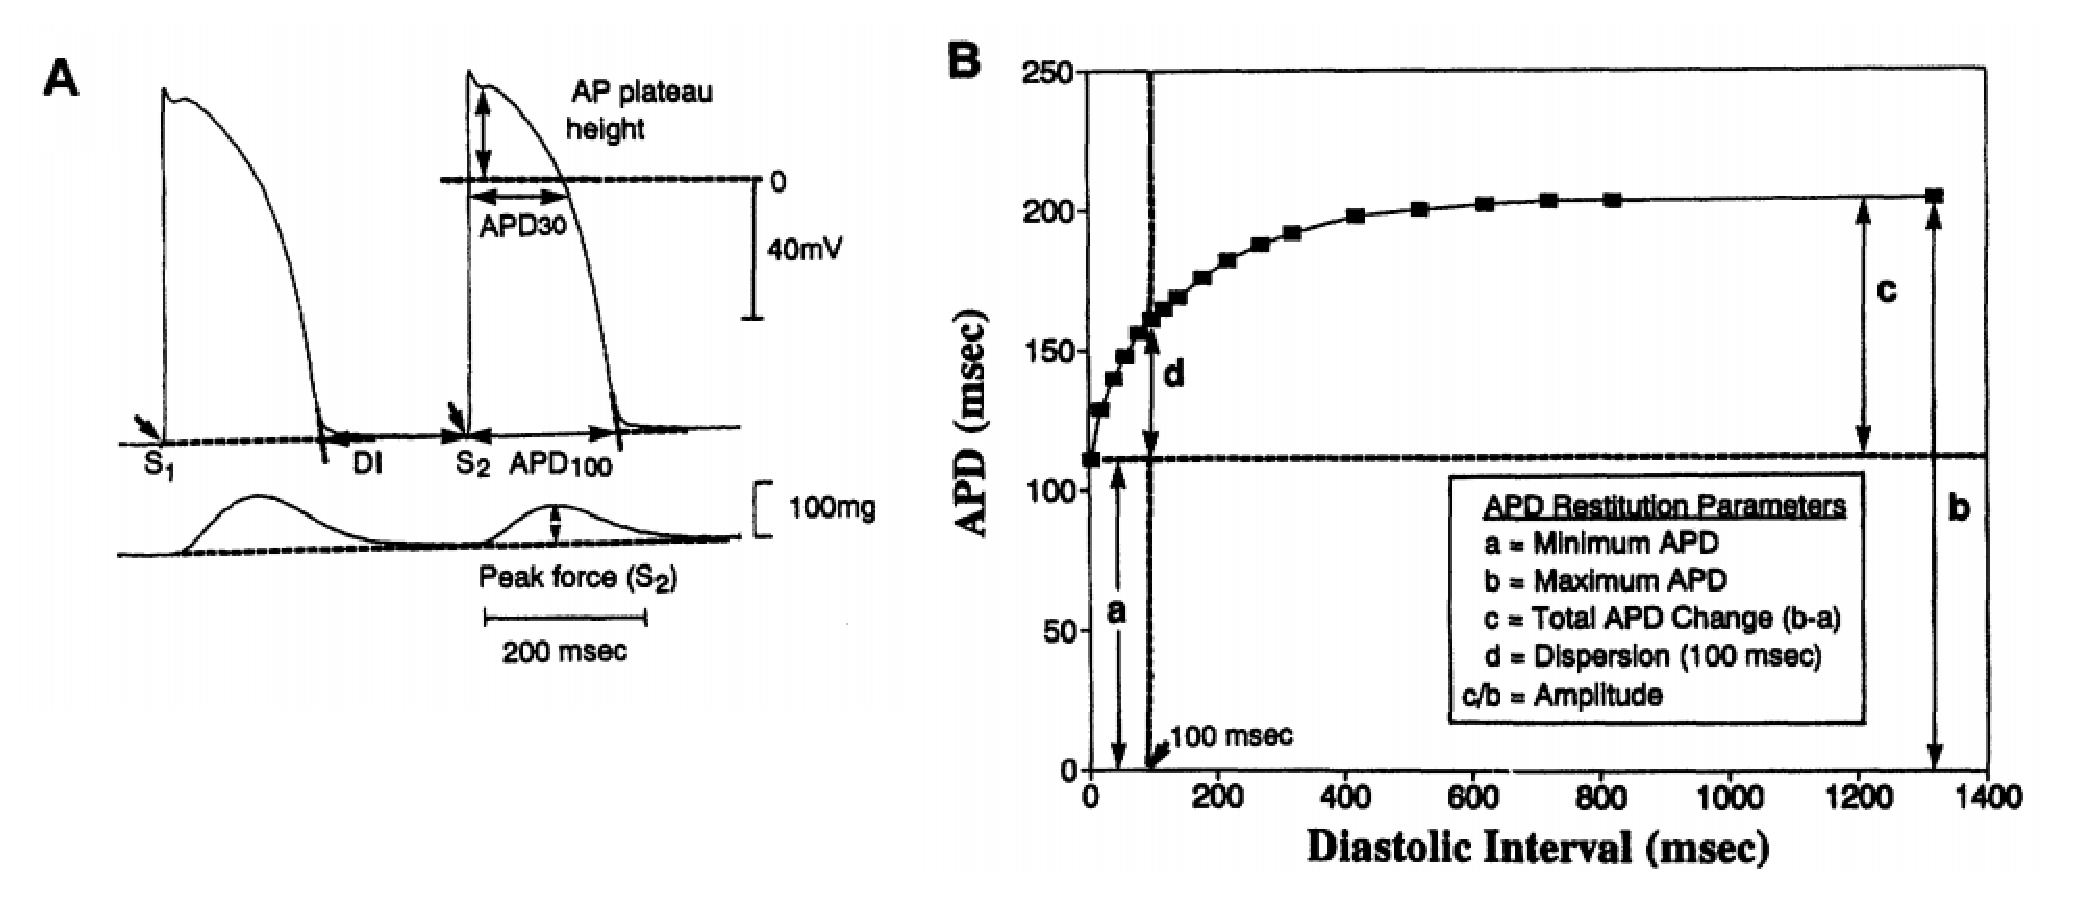
\includegraphics[height=4cm,
 angle=0]{./images/APD_restitution_protocol.eps}} 
 \caption{APD restitution protocol and its parameters \cite{Kobayashi1992}}
\label{fig:APD_restitution_protocol}
\end{figure}


\subsection{Single cell}

There have been different hypotheses for the isolated cardiac myocyte. The
repolarization is followed by a period in which the slow inward current
($I_{si}$ or $I_\LCC$) need to recover from inactivation, and the outward
current decays to its resting value. So, if the next beat disturbs these
current, it may cause a shorter APD \citep{boyett1978}
\begin{enumerate}
  \item Inactivation of the L-type calcium channel, i.e. in the next premature
  beat, LCC has not been fully recovered yet from inactivation so less inward
  current \citep{gettes1974}. \citep{beeler1977rap} estimated the time-constant
  of recovery is about 50 ms at 37$^\circ$C.
  
  \item Activation of the potassium outward current ($I_x$): outward current is
  still large at the next beat \citep{deHemptinne1971, hauswirth1972}. 
  \citep{beeler1977rap} estimated the time-constant of recovery is about 200 ms
  
NOTE: The first two are called 'membrane recovery' hypotheses. The next two,
given below, are called 'ion accumulation' hypotheses.

  \item $[\Ca]_\myo$ is still high at the next beat, so the electrochemical
  gradient for the $I_\LCC$ is lower, i.e. reducing the current
  \citep{reuter1973dcc}

  \item The outward current is increased through an effect on the permeability
  of the membrane potassium \citep{meech1976, bassingthwaighte1976} 
\end{enumerate}

\begin{figure}[hbt]
 \centerline{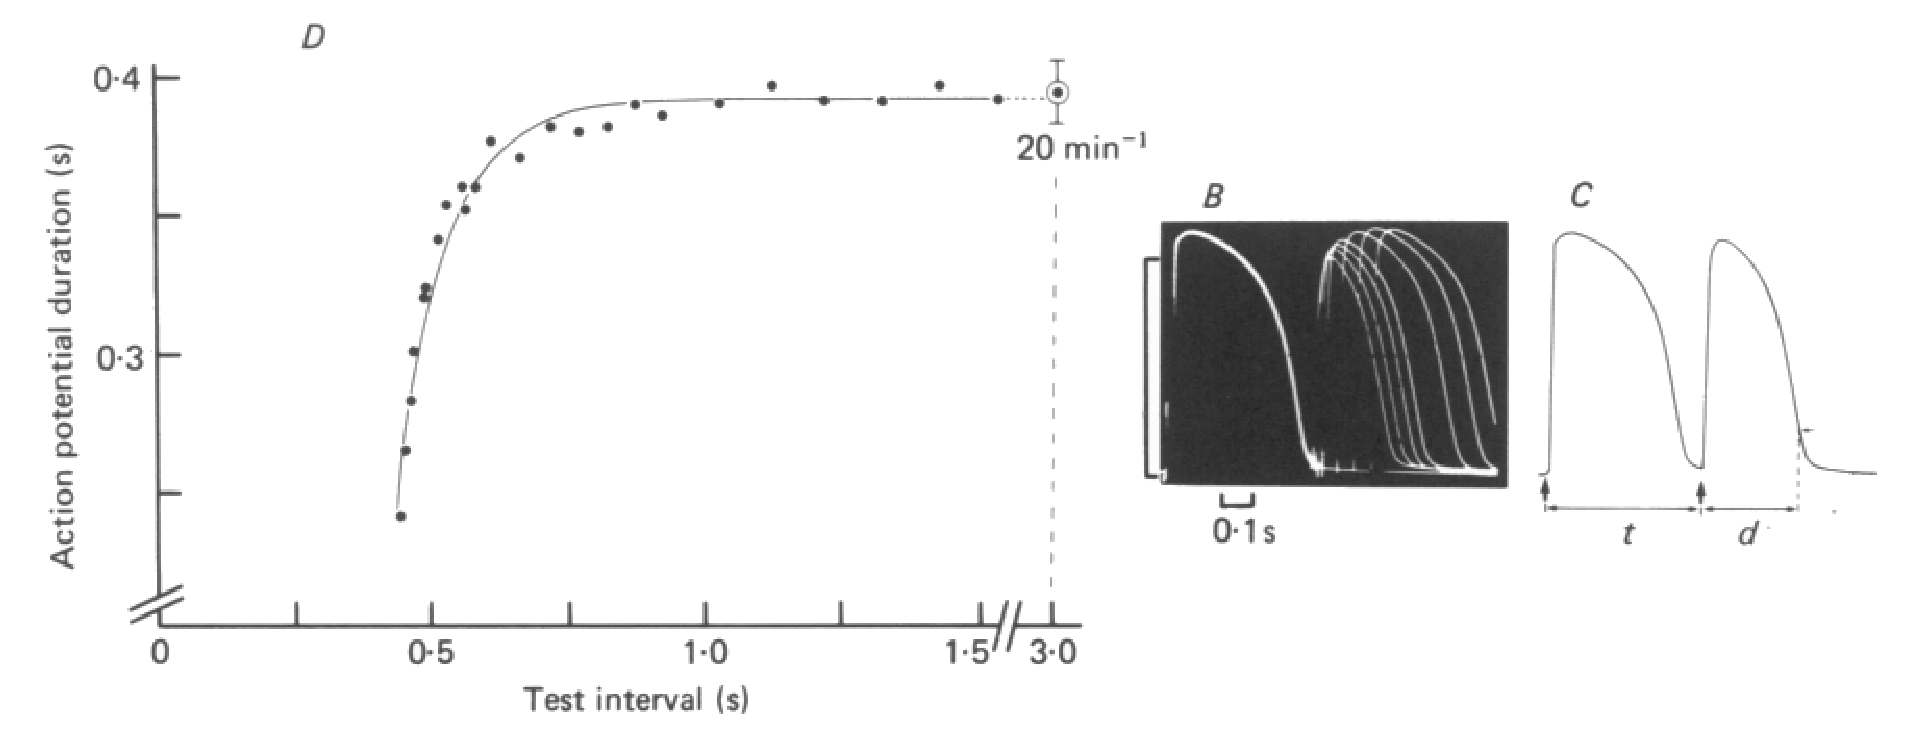
\includegraphics[height=4cm,
 angle=0]{./images/APD_restitution.eps}} 
 \caption{APD restitution: The next APD based on the interval from the previous
 heart beat \cite{boyett1978}}
\label{fig:APD_restitution}
\end{figure}


\citep{Kobayashi1992}


%%% Local Variables: 
%%% mode: latex
%%% TeX-master: "mainfile"
%%% End: 

\chapter{Myocytes (Muscle cells)}
\label{chap:myocyt-muscle-cells}


% In Chapter \ref{chap:nerve-signals}, we have learnt that neurons
% communicate to each other via gap junctions called {\it synapses}. The
% question is how nerve cells communicate to other types of cells, in
% the PNS? - The nervous system communicates with the muscle cells in a
% similar way via {\bf neuromuscular junction} (or myoneural junction)
% and the mating cells are excitable cells. In this chapter, we will
% study a type of excitable cells - the muscle cell or {\it myocyte}
% ({\it myo-} = muscle, {\it -cyte} = cell).

\section{Types of muscle cells}
\label{sec:types-muscle-cells}


\begin{figure}[htb]
  \centerline{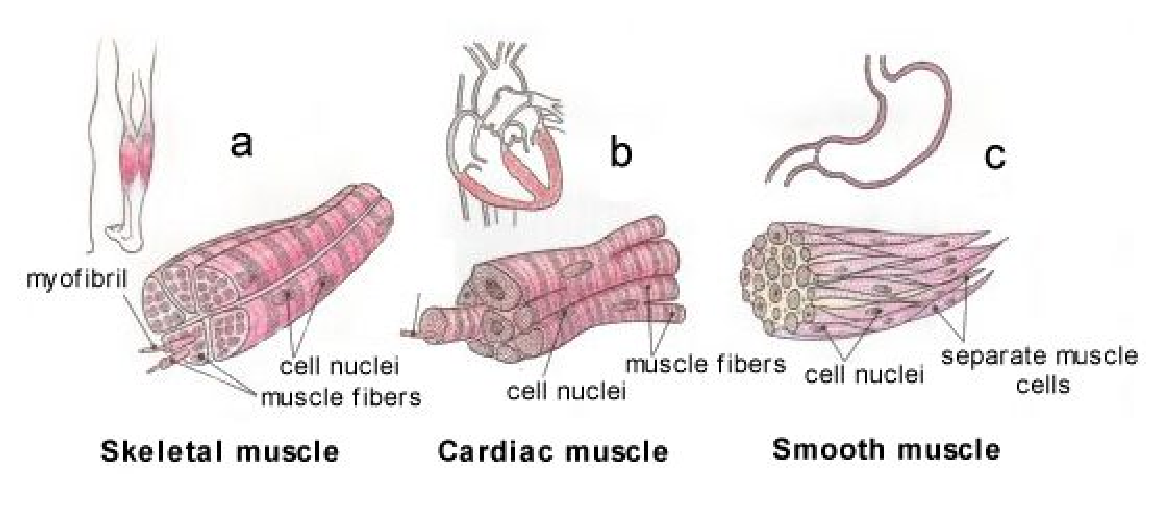
\includegraphics[height=5cm]{./images/muscle_cell_types.eps}}
  \caption{Types of muscle cells}\label{fig:muscle_cell_types}
\end{figure}

A muscle cell, by definition, is an elongated contractile cell that
form the muscle of a body, responsible for movements of the body and
for changes in sizes and shapes of internal organs. 
Along with neurons, the muscle cells are electrically excitable cells
(Sect.\ref{sec:excitable-cells}).

There are two broad types of muscle cells:
\begin{enumerate}
  \item smooth muscle, 
  \item striated muscles: skeletal muscle, cardiac muscle
\end{enumerate}

However, we often classify muscle cells into 3 classes as striated muscles is
further divided into two subclasses: skeletal muscle, and cardiac muscle, based
on the cells' locations\footnote{\url{http://www.brianmac.co.uk/muscle.htm}}, as
shown in Fig.~\ref{fig:muscle_cell_types}.  In practice, the term {\it striated
muscle} is used exclusively to refer to {\it skeletal muscle} where the striated
appearance (i.e. a light band alternate a dark band) is very well organized. 
The term {\it cardiac muscle} is used as-is for the third class of muscle cells
where the striated appearance is much less organized, as shown in
Fig.\ref{fig:muscle_types}.

\begin{figure}[hbt]
 \centerline{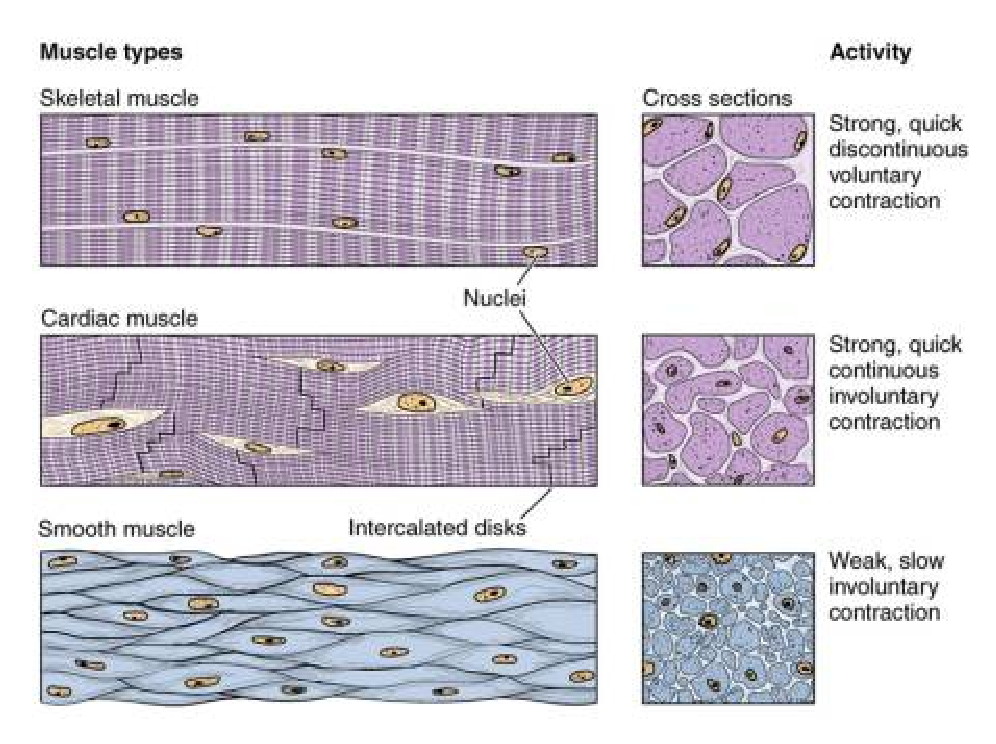
\includegraphics[height=8cm, angle=0]{./images/muscle_types.eps}}
\caption{The three types of myocytes\footnote{\url{http://www.mc.vanderbilt.edu/histology/labmanual2002/labsection1/Muscle03.htm}}}
\label{fig:muscle_types}
\end{figure}

\begin{itemize}
\item smooth muscles: lining the wall of many body's hollow organs
\item skeletal muscle (striated muscles): found in
  junction with the bones (skeleton)
\item cardiac muscles: found in cardiac (the heart)
\end{itemize}


\section{Smooth muscles}
\label{sec:smooth-muscles}

\subsection{Taxonomy}
\label{sec:taxonomy}


\begin{figure}[htb]
  \centerline{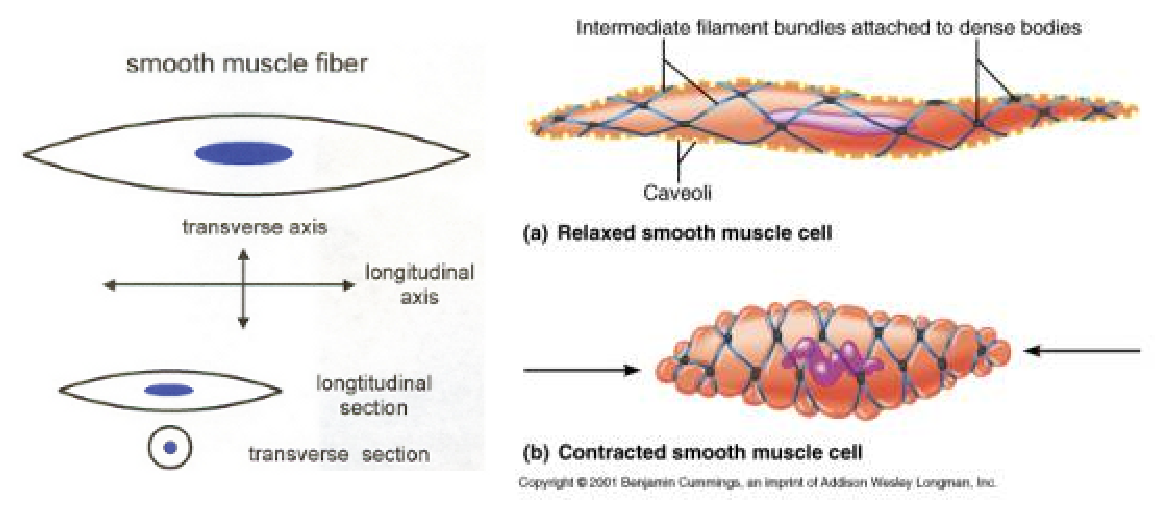
\includegraphics[height=5cm]{./images/smooth_muscle_cells.eps}}
  \caption{(A) spindle-shape, (B) {\it relaxation} and
    {\it contraction} of smooth muscle
    cells}\label{fig:smooth_muscle_cells}
\end{figure}

Smooth muscle cells have
spindle-shape, as shown in Fig.~\ref{fig:smooth_muscle_cells}(A)\footnote{\url{http://education.vetmed.vt.edu/curriculum/vm8054/labs/Lab10/Notes/spindle.htm}}
and is responsible for the contractility of hollow organs (uterus,
gut, stomach, around blood vessels or muscular arteries...).
Fig.\ref{fig:smooth_muscle_cells}(B) shows two states of a smooth muscle
cell (i.e. relaxation and contraction). These are also the common
states in all excitable cells. In terms of taxonomy, a smooth muscle
cell can belong to either {\it single-unit} or {\it multi-unit} (or
{\it visceral}) cells.

% nomenclature
{\bf Single-unit smooth muscle cells} are smooth muscle cells that
operate coordinately as a unit. Particularly, they are electrically
coupled (by many gap junctions) in that the electrical stimulation of
one cell is followed by the stimulation of the adjacent single-unit
smooth muscle cells. This forms a wave-like contraction, aka
{\bf peristalsis}, and can be initiated by a pace-maker (i.e. a smooth
muscle cell that exhibits a spontaneous depolarization).  The second
type, {\bf multi-unit smooth muscle cells} are not electrically
coupled, i.e. the activation of one cell is independent from another
adjacent cells as there are only a few gap junctions between them and
synaptic gaps are narrow.

\begin{itemize}
\item Single-unit group (the most common): line the hollow organs
  (gut, uterus...).
\item Multi-unit group: line the large-airways to the lungs and the
  large blood vessels, ciliary muscle, iris, arrector pili.
\end{itemize}


\begin{figure}[htb]
  \centerline{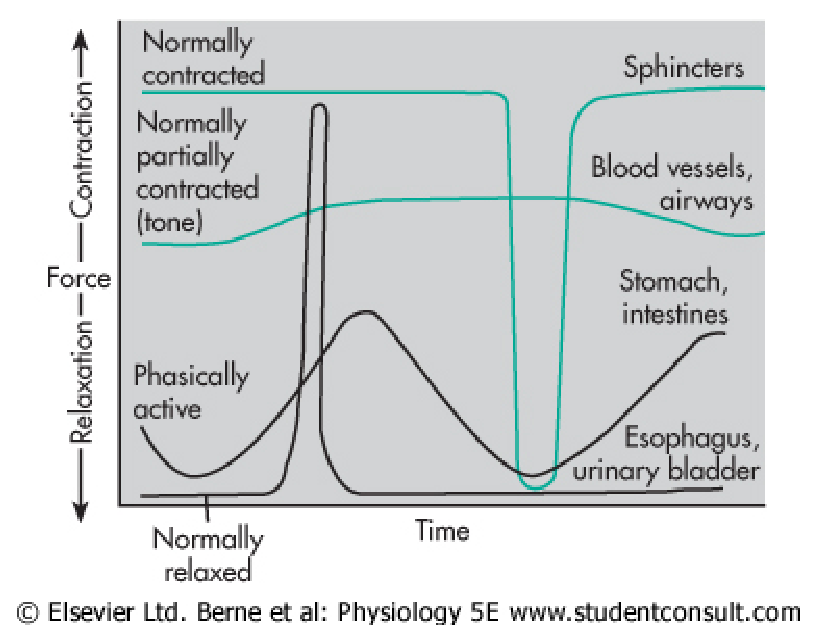
\includegraphics[height=5cm]{./images/smooth_muscle_cells_rhythmic_contraction.eps}}
  \caption{Some contractile activity patterns exhibited by smooth
    muscle cells}\label{fig:rhythmic_contraction_SMC}
\end{figure}

Another consideration for classification is contractile pattern,
i.e. the response to depolarizing in high \ce{K+} solution with
different patterns. As shown in
Fig.\ref{fig:rhythmic_contraction_SMC}, {\it tonic smooth muscle}
cells contract and relax slowly (e.g. vascular smooth muscle). The
{\it phasic smooth muscle cells} contract and relax quickly (e.g. gut
smooth muscle). Phasic smooth muscles are single-unit muscles.  There
are different ways to stimulate a smooth muscle cells: (1) from the
nerve cells, (2) from neighboring cells, (3) hormones.

% that normally relax and contract only when having electrical signals
% are called {\bf phasic smooth muscles}, e.g. smooth muscle in the
% gastrointestinal and urogenital tracts. Phasic smooth muscles are
% single-unit muscles. On the other hands, the smooth cells that
% continuously active (i.e. contract) and relaxed only when there is a
% signal is termed {\bf tonic smooth muscles}.


\subsection{Structure}
\label{sec:structure-2}


% organizing
Smooth muscle cells are organized into 2 or 3 layers. One layer run
circularly around the lumen, one runs longitudinally along the length
of the organ. And in the stomach, there is another layer that run
diagonally or obliquely. The adjacent cells have closely mechanical
and functional linkage through the gap junctions, as shown in
Fig.\ref{fig:SMC_linkage} (A). 

\begin{figure}[htb]
  \centerline{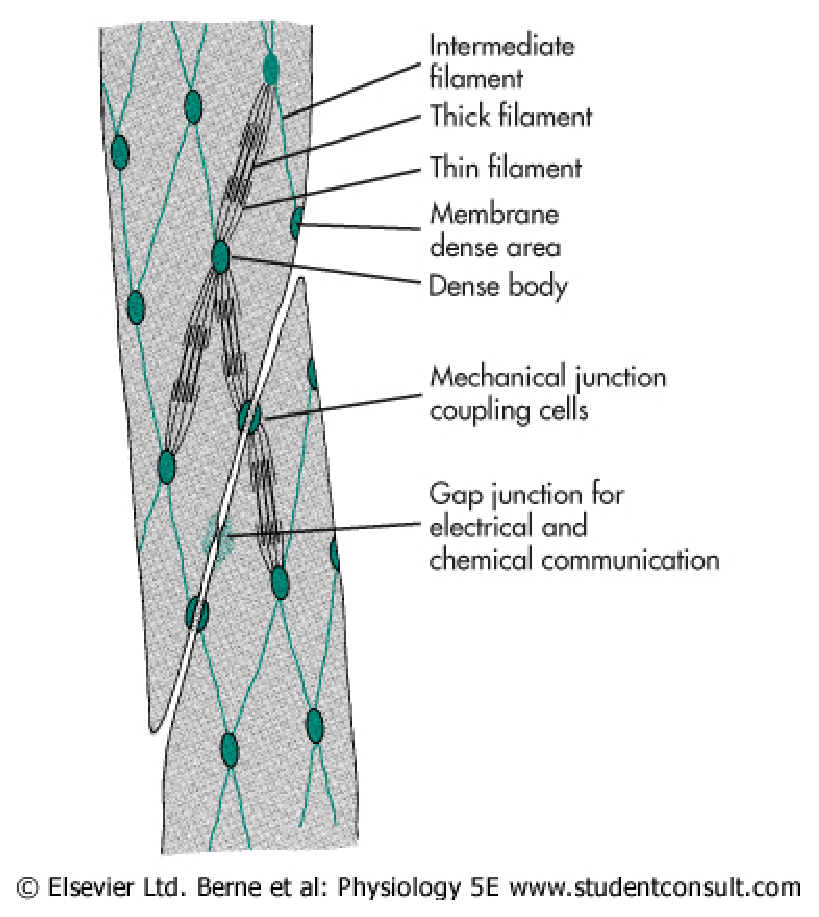
\includegraphics[height=7cm]{./images/muscle_cell_linkage.eps}
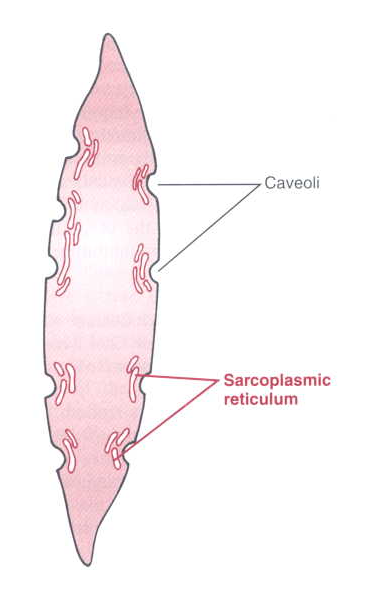
\includegraphics[height=7cm]{./images/Caveolae_SMC.eps}}
\caption{(A) apparent organization of cell-to-cell contacts, (B)
  smooth muscle cell structure}\label{fig:SMC_linkage}
\end{figure}


% internal structure
Now, we look at the ultrastructure of a smooth muscle cell.  In muscle
cells, the {\bf sarcoplasm} is the cytoplasm, and the {\bf sarcolemma}
is the biomembrane.  As shown in Fig.\ref{fig:SMC_linkage}(B), on the
{\bf sarcolemma}, there is the presence of
{\bf
  caveoli}\footnote{longitudinal
  rows of tiny saclike inpocketings},
the invaginations of the smooth muscle membrane allowing the ion
channels to form a dyadic subspace (junctional space) with the
{\it sarcoplasmic reticulum} (SR) - the smooth endoplasmic reticulum
of muscle cells. SR locates sparsely and throughout the smooth muscle
cell. This is analogous to the T-tubules in the striated muscle which
is described in the next section.  Such junctional space provide
electrical links between the SR and caveoli to mediate the release of
\ce{Ca^2+} triggered by the influx of \ce{Ca^2+} through ion channels
on caveoli.

% resting potential
\textcolor{red}{In smooth muscle cells, the resting potential is in
  the range $-60$ to $-40$ mV}.
The action potential (AP) in smooth muscle cells shows a wide range of
properties, some being less \ce{Ca^2+} dependent while others being
more so - very much like that in cardiac AP with a plateau
corresponding to a period of \ce{Ca^2+}
entry\footnote{\url{http://www.mona.uwi.edu/fpas/courses/physiology/muscles/Smooth_Muscle.htm}}.


\begin{figure}[hbt]
  \centerline{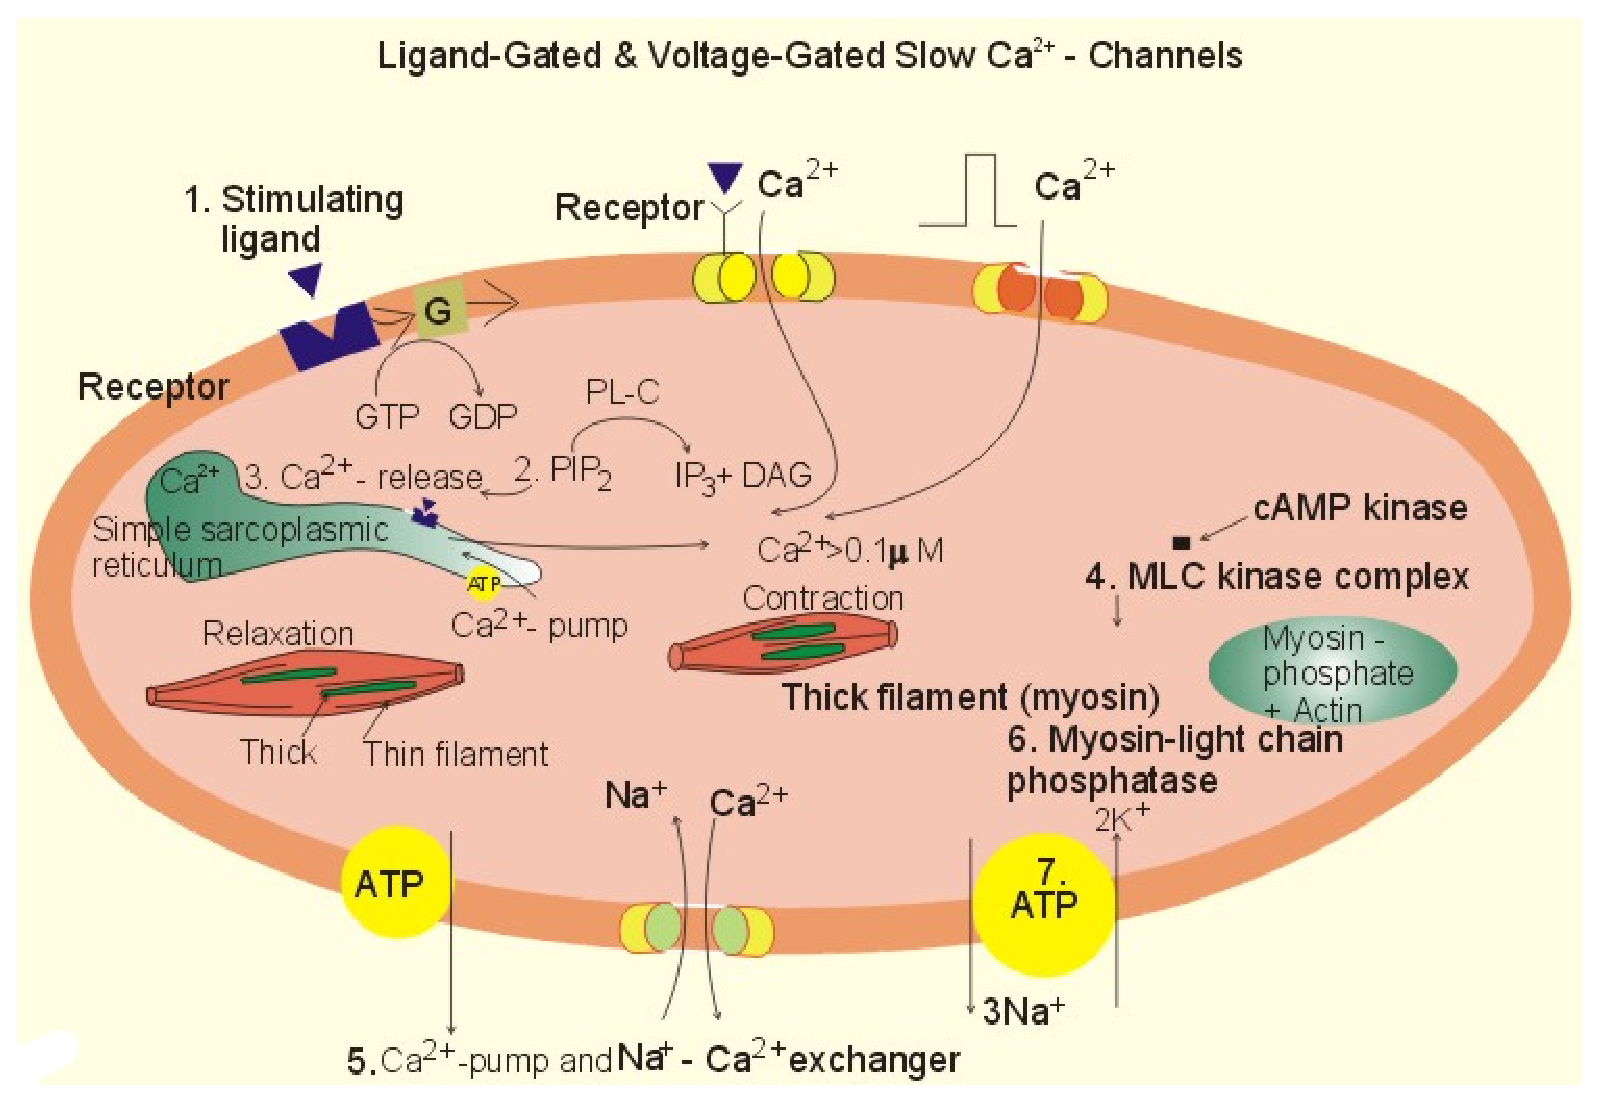
\includegraphics[height=6cm,
    angle=0]{./images/smooth_muscle_components.eps}}
\caption{The excitation-contraction of smooth muscle cells}
\label{fig:smooth_muscle_structure}
\end{figure}


The network of SRs serves as the intracellular reservoirs for
\ce{Ca^2+} (will talk about the role of \ce{Ca^2+} in cell signalling
chapter later). As a reservoir for intracellular \ce{Ca^2+}, there
should be some gates in SR for calcium releasing. Those gates are
\begin{itemize}
\item \ce{Ca^2+}-activated Ryanodine-sensitive \ce{Ca^2+} release
  channels called {\bf ryadonine receptor} ({RyR}). There are 3 types
  RyR(1-3).

\item \ce{Ca^2+}-activated
  {\bf inositol 1,4,5-triphosphate ($IP_3$)}-sensitive \ce{Ca^2+}
  release channels called IP3R. There are 3 types IP3R(1-3). 
\end{itemize}
In cardiac cells, the mechanism for calcium elevation in excitable
cells is the \ce{Ca^2+}-induced \ce{Ca^2+} released
(\hyperref[sec:cicr]{CICR}). However, in contrast to cardiac cells,
the coupling between RyR2 and L-type \ce{Ca^2+} channels in muscle
cells is not obvious and results in a ``loose
coupling''~\cite{amberg2006cicr}.


In essence, when \ce{Ca^2+} channels in the caveoli open as the result
of action potential, there is an increase in local intracellular
\ce{[Ca^2+]} in the junctional space between the caveoli and the
SR. This will trigger the activity or open the gates of RyR in SR so
that the \ce{Ca^2+} inside the SR can be released. This, in turns,
continue to increase the [\ce{Ca^2+}] near the junctional space; and
positively feedback on more \ce{Ca^2+} release. However,
interestingly, not all \ce{Ca^2+} inside the SR are released.
\textcolor{red}{The release of \ce{Ca^2+} from the SR simultaneously
  increase the \ce{[Ca^2+]}, however, only 50-60\% or \ce{Ca^2+} is
  released}~\cite{bassani1995fsr}.

$IP_3$-gated \ce{Ca^2+} channel is activated by $IP_3$, which is
produced when hormone(s) bind to the various \ce{Ca^2+}-mobilizing
receptors on the sarcolemma. Further, IP3-receptors are also activated
by CICR and that there can be bidirectional communication between RyR
and IP3-receptors. Read more in the next chapter
\footnote{\url{http://www.ursa.kcom.edu/LectStreams/Other/DesMoines/SmMuscle_DesMoines_files/frame.htm}}

% A region near the nucleus is filled with smooth endoplasmic reticulum
% (SER) and lots of
% mitochondria\footnote{\url{http://www.cytochemistry.net/microanatomy/muscle/smooth_muscle_2001.htm}}.
% Mitochondria is the factory for ATP-manufacturing, while SER is the
% storage place for \ce{Ca^2+}. In myocytes, SER is given the name
% {\bf sarcoplasmic reticulum} (SR) and the membrane is called
% {\bf sarcoplasm}.

% \begin{figure}[htb]
%   \centerline{\includegraphics[height=8cm]{./images/SMC_contraction_relaxation.eps}}
%   \caption{contraction/relaxation in smooth muscle
%     cells}\label{fig:SMC_contraction_relaxation}
% \end{figure}





\subsection{Electrophysiology: smooth muscle hyperpolarization (EDHF)}
\label{sec:EDHF}

Consider a blood vessel, with the inner layer is endothelial cells, and then
next is (vascular) smooth muscle cells
\begin{verbatim}
cell layer: (vascular) smooth muscle cells
cell layer: endothelial cells
-------------------------------
--------------------(blood flow)
-------------------------------
cell layer: endothelial cells
cell layer: smooth muscle cells
\end{verbatim}


Smooth muscle hyperpolarization is important to cause the cells to relax,  thus
allowing the blood vessel to expand in diameter. Vasolidators refers to 'things'
that widening the blood vessels.

Examples of vasolidators:
\begin{itemize}
  \item nitric oxide (NO) is recognized as the primary factor in arteries
  
  However, NO is not the only vasolidator.
  When NO and Prostacyclin (Vasodilators) are inhibited there is still another
  factor causing the vessels to dilate.
  
  \item recent evidences: 'things' released from endothelium cells, they are
  collectively called Endothelium-derived vasodilator (or {\bf
  endothelium-derived hyperpolarizing factor} (EDHF)
  
%   refers to a substance and/or electrical signal that is generated or synthesized in and released from the endothelium; its
% action is to hyperpolarize vascular smooth muscle cells.

EDHF was suggested to be 
  \begin{enumerate}

    \item $\K$ released from endothelial cells during ACh stimulation
    (Sect.\ref{sec:Acetylcholine})

NOTE: the hyperpolarization of these cells to ACh was abolished in the presence
of apamin and charybdotoxin, but not apamin and iberiotoxin.
NOTE: Charybdotoxin block $\Ca$-activated $\K$ channels
(Sect.\ref{sec:K(Ca)_antagonists}).

    \item 
  \end{enumerate}
 
\end{itemize}


Smooth muscle contractile activitycorrelates well with the level of free
intracellular Ca2+ available to the contractile apparatus.

Under physiological conditions, membrane potentials of smooth muscles lie
positive to the reversal potential for K+(Erev K $\approx$ -80 to -90 mV).

Voltage-gated, Ca2+-independent K+ (Kv) currents are present in all smooth
muscles.




\subsection{Small airways smooth muscle}
\label{sec:smooth-muscle-small-airways}

Small airways are a major site of airflow limitation in chronic obstructive
pulmonary disease (COPD).

Once believed to be just a contractile tissue, airway smooth muscle (ASM) is
instead characterized, in addition to contraction, by many other biological and
functional properties including regulation of bronchomotor tone, perpetuation
and amplification of airway inflammation, as well as active participation in
structural remodeling of the bronchial wall.
ASM contraction and proliferation significantly participate in the development
and progression of asthma.

%http://www.sciencedirect.com.mutex.gmu.edu/science/article/pii/S0954611108000966

Agonist-induced increase in $\Ca$ occur in the form of propagating calcium
oscillation. In airway smooth muscle cells, at room temperature (25$^\circ$C),
agonist-induced or IP3-induced calcium oscillation can be blocked by IP3R
antagonist (2-aminoethoxydiphenyl borate (2-APB)) and induce airway relaxation,
while using ryanodine (an RYR2 antagonist) has no significant effect, at any
concentration. The second RyR antagonist (tetracaine) can block agonist-induced
$\Ca$ oscillations at high concentration, but not IP3-induced $\Ca$ oscillation
at any concentration \citep{bai2009}. This suggested that agonist-induced $\Ca$
oscillation in mouse small airway smooth muscles are primarily mediated by IP3R.





\section{Skeletal muscles}
\label{sec:skeletal-muscles}

\begin{figure}[hbt]
  \centerline{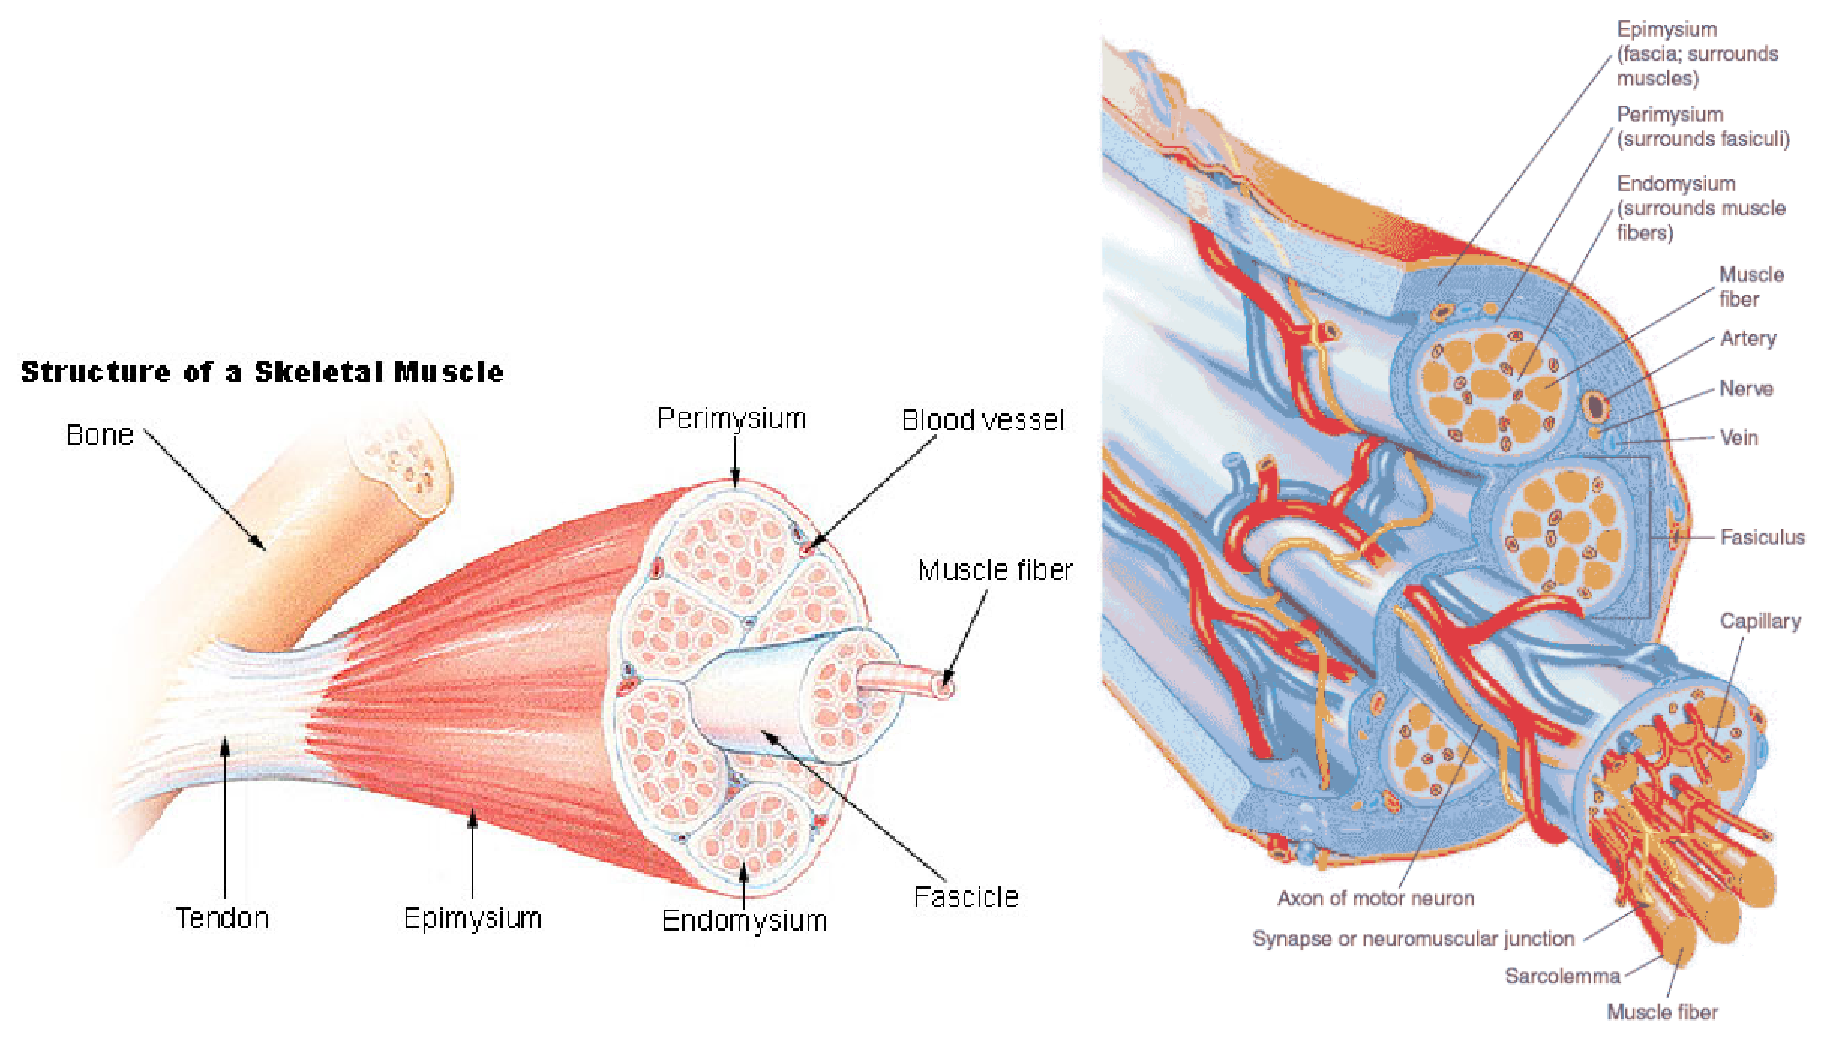
\includegraphics[height=7cm,
    angle=0]{./images/skeletal_muscle_tissue.eps}}
  \caption{The skeletal muscle tissues}
\label{fig:skeletal_tissue}
\end{figure}

Skeletal muscle tissues (striated muscle) are {\it found attached to bones}
(hence the name skeletal)  by a bundle of collagen fibers \footnote{Collagen in
Greeks means ``glue
  producer''}  - special proteins - known as
{\it
tendons}\footnote{\url{http://www.web-books.com/eLibrary/Medicine/Physiology/Muscular/Skeletal_Structure.htm}}.
Its contraction and excitation support the movement of the human body, hence
provide the organisms a wide range of physical capabilities.

The skeletal muscle tissues is sheathed by a membrane called {\bf epimysium}. A
skeletal muscle tissue is divided into clusters, called {\bf muscle fasicle},
along with other organelles (artery, nerve, vein).


Each fasicle is a bundle of skeletal muscle fibres  (ranging anywhere between 10
to 100 or more). Each fasicle is enclosed by a type of connective tissue called
{\bf perimysium}, keeping skeletal muscle fibres together. Recent advances in
muscle physiology suggest that perimysium plays a role in transmitting lateral
contractile movements\footnote{\url{http://en.wikipedia.org/wiki/Perimysium}}.
Each skeletal muscle fibre, in turns, is enclosed by a layer of connective
tissues called {\bf endomysium}, as shown in Fig.~\ref{fig:skeletal_tissue}.

{\bf Skeletal muscle fibres} have more than one nucleus. with the nuclei
locating near the sarcolemma. \footnote{due to the multinuclei of the cell, we call it fibre
rather cell}
These long, cylindrical, multinucleated cells are also called myofibers.
  
Each fibre has a cylindrical, elongated
shape with range in length from 1 to 40mm and in diameter from 0.01 to
0.1 mm. {\it Sartorious muscle} - the longest muscle in human body -
contains a single fibers with about 30cm
long\footnote{\url{http://en.wikipedia.org/wiki/Sartorius_muscle}}.
Further, each fibre is distinguished by an alternating dark and light
bands which are {\bf myofibrils}. This is the origin of the
description ``striated''.  

All skeletal muscle fibres are in a parallel arrangement. As shown in
Fig.~\ref{fig:skeletal_fibre}, each fibre is filled with many longitudinal
parallel-arranged small fibres, called {\bf myofibril}. Myofibrils are 1-2$\mu
m$ in diameter, and have alternate light (I-band) and dark bands (A-band).
  

% \begin{figure}[htb]
%   \centerline{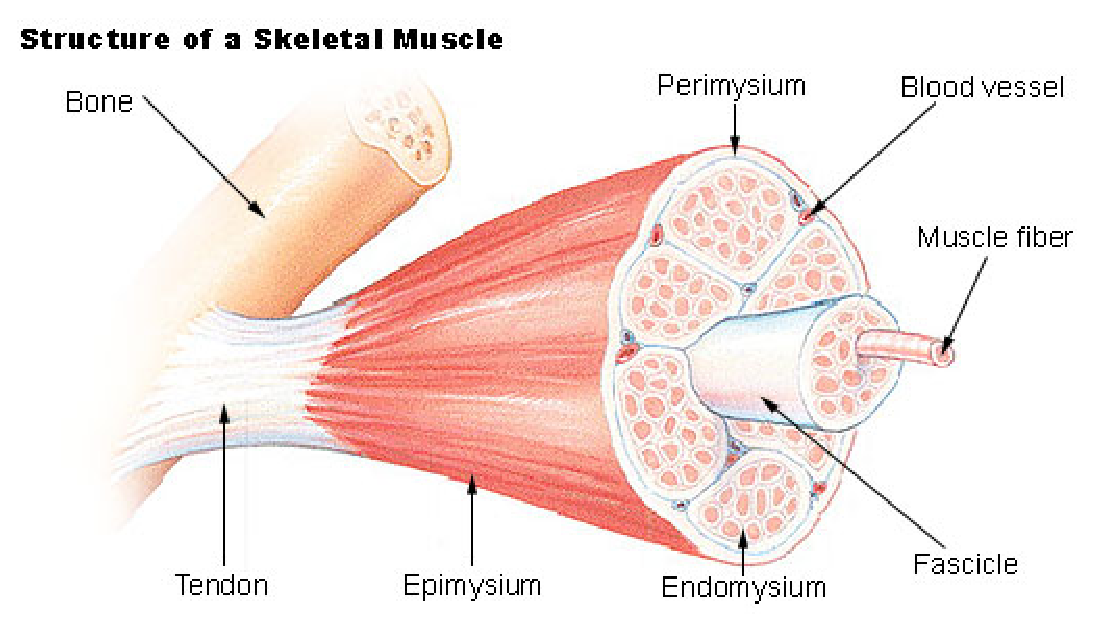
\includegraphics[height=5.5cm]{./images/skeletal_muscle.eps}}
%   \caption{Skeletal muscle}\label{fig:skeletal_muscle}
% \end{figure}
% As shown in Fig. \ref{fig:skeletal_tissue}, a single
% skeletal muscle cell is cylindrical, elongated fibre. It can be extremely
% short or long.  
% Structurally, each skeletal muscle (NOTE: not skeletal cell),
% surrounding by a membrane called {\bf epimysium}, is composed of many
% compartments, called {\bf fasicles} (a bundle of fibre). Each fasicle
% is, in turn, composed of many muscle cells (muscle fibre). Each muscle
% fibre is enclosed by a layer of connective tissue called
% {\it endomysium}.
% Surrounding a fasicle is a thin layer of connective tissues called
% {\bf perimysium}, keeping muscle fibres together. 

\begin{figure}[hbt]
 \centerline{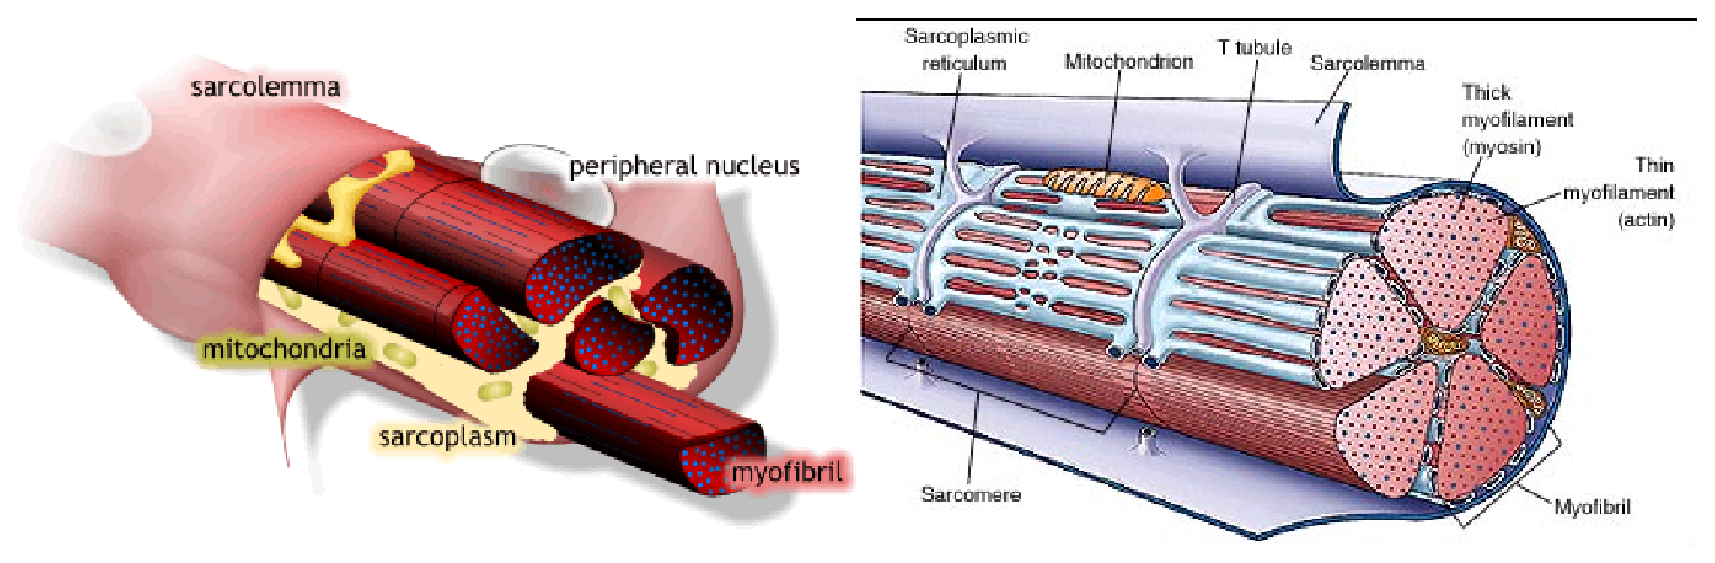
\includegraphics[height=4cm, angle=0]{./images/skeletal_fibre.eps}}
\caption{A single skeletal fibre}
\label{fig:skeletal_fibre}
\end{figure}

%  (hence the
% name striated = having parallel lines or grooves on the surface). 

\subsection{Myofibrils}
\label{sec:myofibrils}

Muscle fibres are typically 2-3 cm long and 100$\mu$m in
diameter. Fibers are built from smaller unit called {\bf myofibrils}
of 1-2$\mu$m in diameter which primarily contains thick myosin
filament (12-18 nm in diameter) and thin actin filament (5-8 nm in
diameter)\footnote{\url{http://www.ks.uiuc.edu/Research/telethonin/}}.

\begin{figure}[hbt]
  \centerline{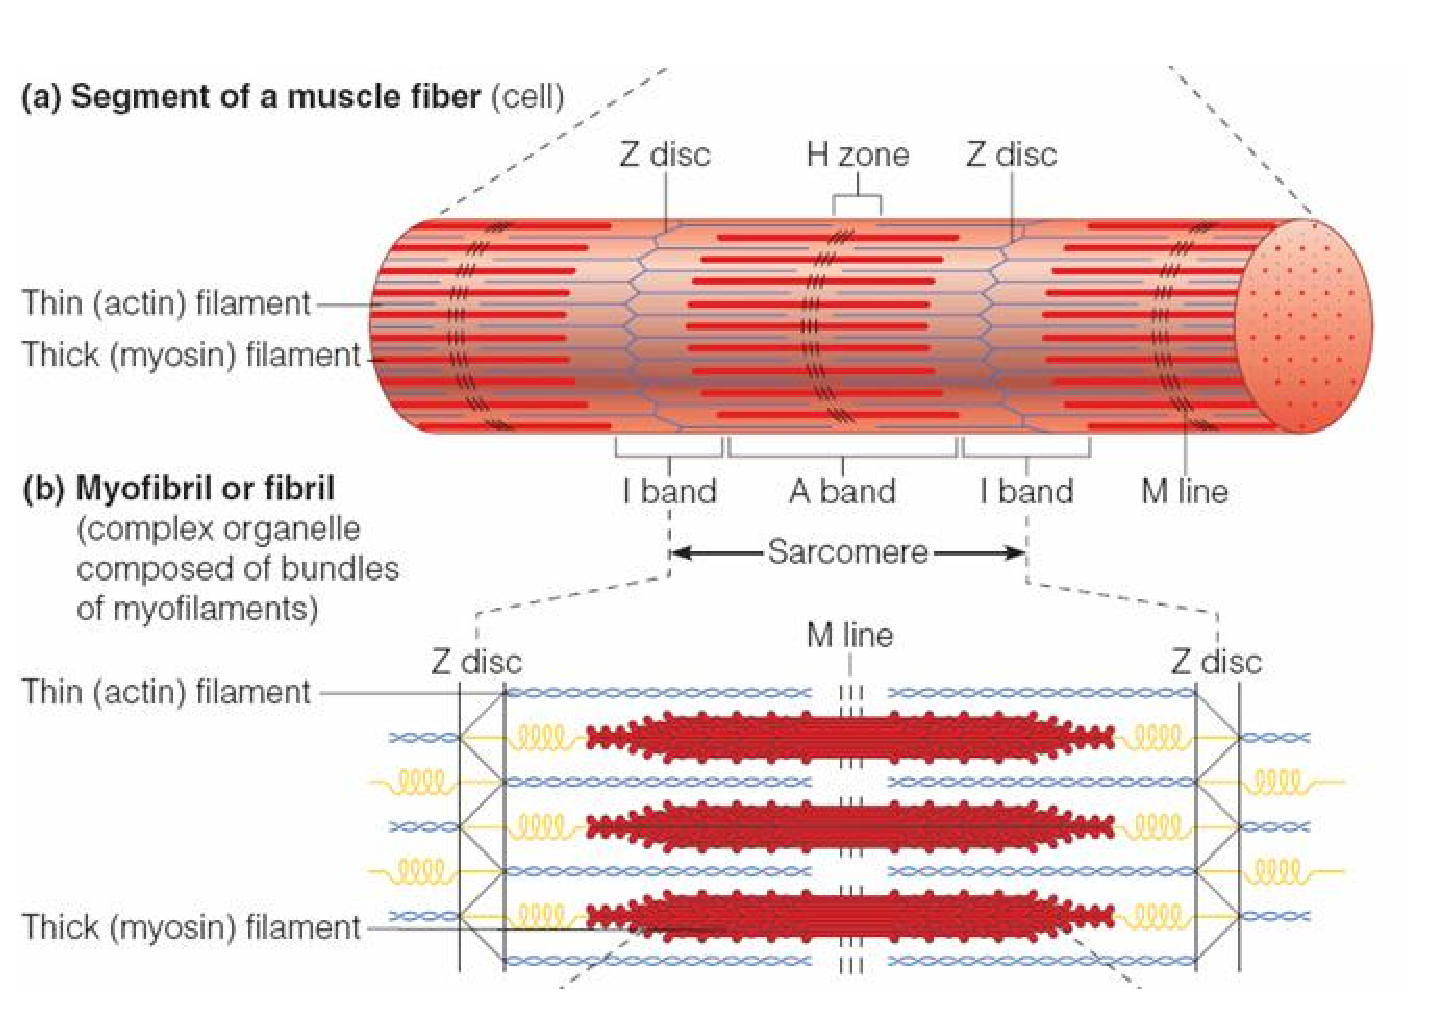
\includegraphics[height=6cm,
    angle=0]{./images/skeletal_muscle_fibre.eps}}
\caption{Myofibril\footnote{\url{www.shoppingtrolley.net/skeletal muscle.shtml}}}
\label{fig:skeletal_muscle_fibre}
\end{figure}

The skeletal muscles contract via the shortening of muscle fibres, or
microscopically, the shortening of {\it myofibrils}. To understand how
myofibrils contract, we have to know its structures. As shown in Fig.
\ref{fig:skeletal_muscle_fibre}, 
\begin{itemize}
\item the light bands are the thin filaments (primarily protein
  actin), held in place by {\it nebulin filaments}

\item the dark bands are the thick filaments (primarily protein
  myosin), held in place by {\it titin filaments}
\end{itemize}

Below are the two principal types of proteins that form the myofibril.
\begin{enumerate}
\item myosin: $1.5\mu m$ long, $15nm$ in diameter
\item actin: $1\mu m$ long, $5nm$ in diameter
\end{enumerate}

Myofibrils then are organized into subunits (segments) known as
{\bf sarcomeres} (Greek sárx = "flesh", méros = "part") which is
limited by two very dark colored bands known as {\bf Z-lines} (or
Z-disc, Z-border - from the German word ``Zwischenscheibe'', mean
between). All sarcomeres are perfectly aligned to give a striated
appearance from the electron microscopy. 

{\bf Z-disc}: They are dense of protein discs that do not easily allow
the passage of light. 

Between the two Z-disc of a sarcomere, the area is divided into 
\begin{itemize}
\item two lighter colored at the two ends, called I-band (form the
  word isotropic - uniformly in all direction)
\item the darker colored at the center, called A-band (from the word
  anisotropic - the myosin heads are in two different directions)
\end{itemize}
The T-tubule, the membrane invagination, is present in the junction of
A-band and I-band.


{\bf NOTE}: The light or dark color is caused by whether the light can
go through the object easy or difficult. The thick filament, in the
A-band, restrict the passage of light, thus result in a dark color.


\begin{figure}[htb]
  \centerline{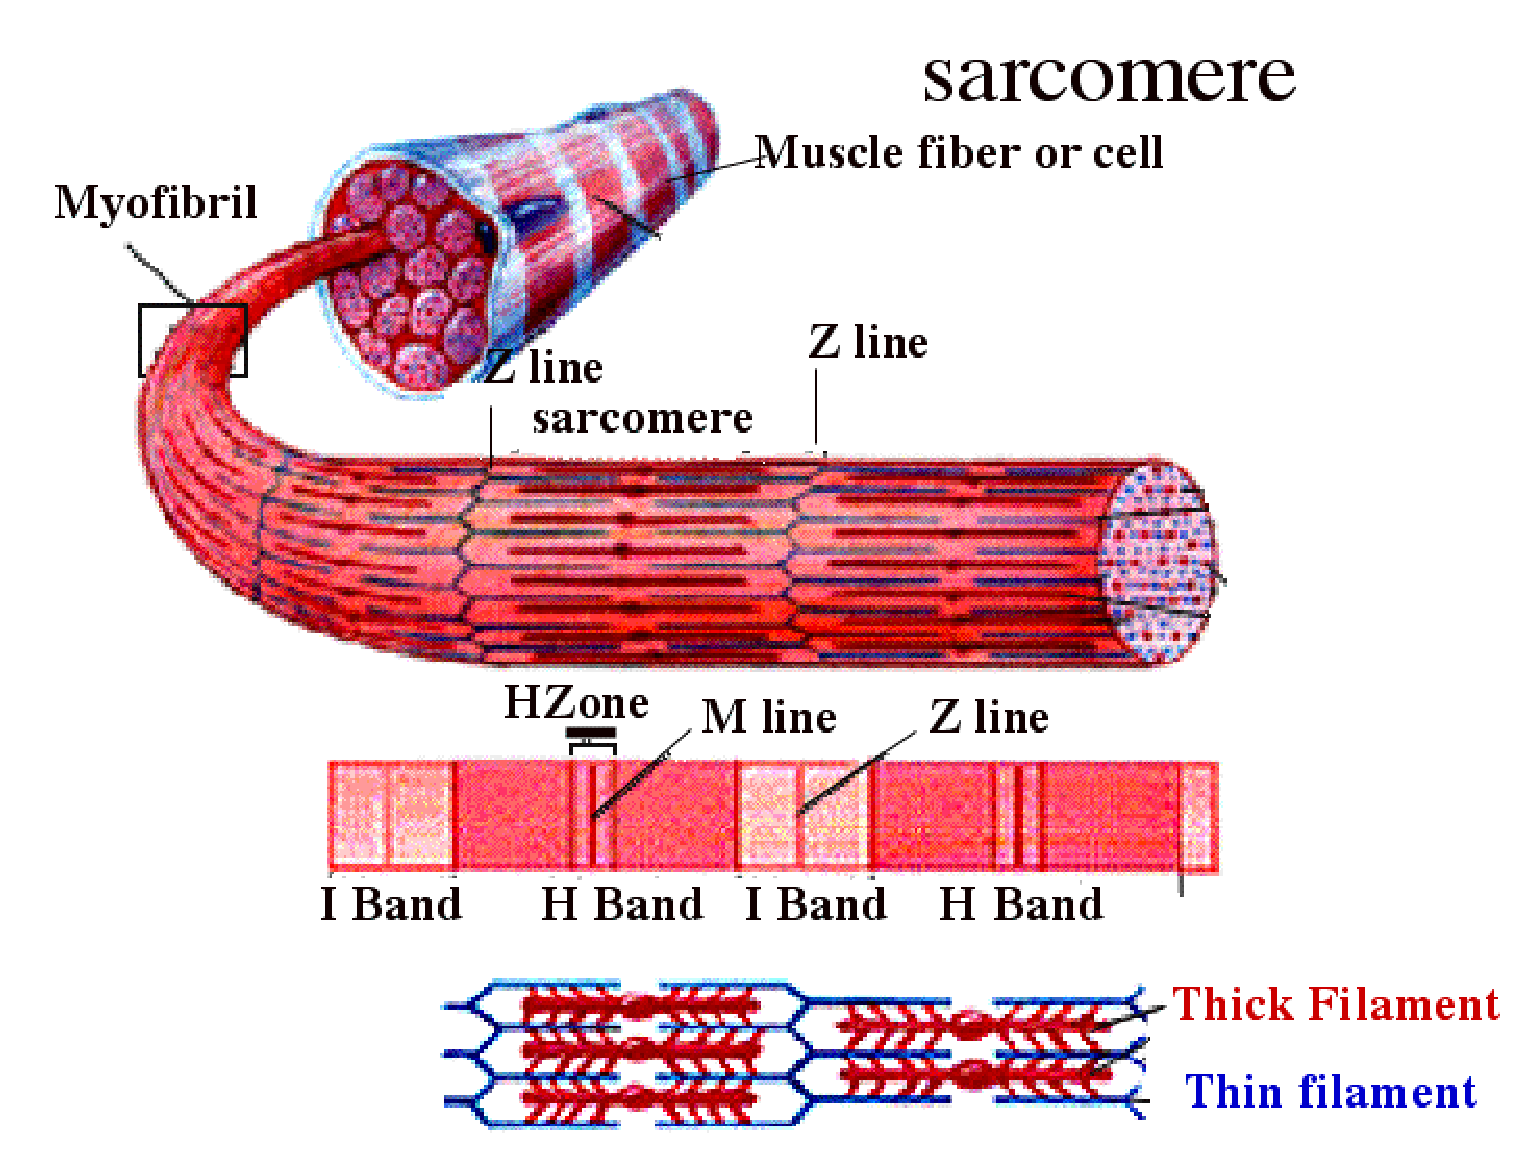
\includegraphics[height=7cm]{./images/sarcomere_0.eps}}
  \caption{Sarcomere (a unit of myofibrils)}\label{fig:sarcomere}
\end{figure}

In the center of the dark A-band, there is a lighter region, known as
{\bf H-zone} (or H-band; from the German ``Heller'' means bright). In
addition, the center line of A-band is a dark line known as
{\bf M-line} (from the German word ``Mittel'' means the middle of the
sarcomere). M-line is also
the center of the thick myosin filament. From the M-line, the myosin
heads stretch out toward the actin, but not in contact, as shown in
Fig.~\ref{fig:sarcomere_structure}. Only when the myofibril contract,
do myosin heads come into contact with actin.

\begin{figure}[htb]
%  \centerline{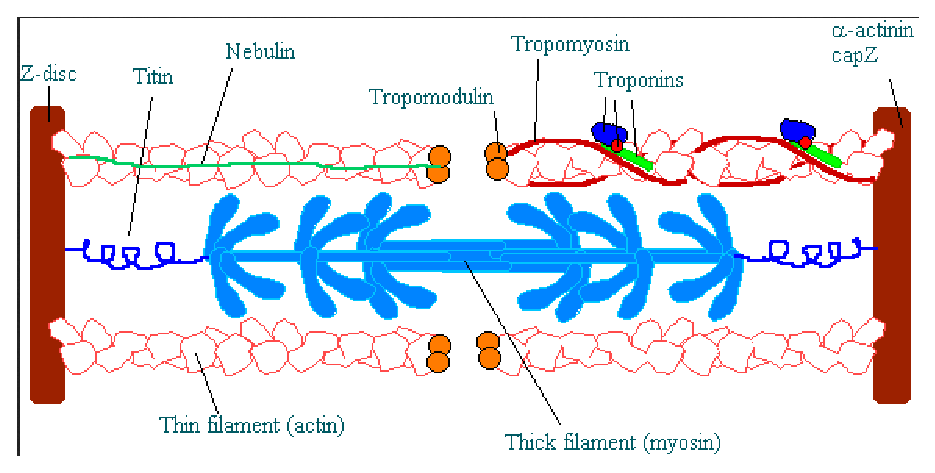
\includegraphics[height=4cm]{./images/sarcomere.eps}}
  \centerline{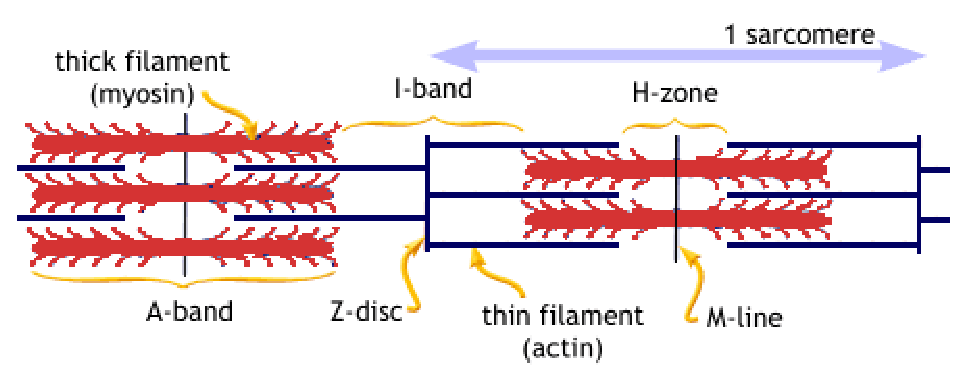
\includegraphics[height=4cm]{./images/sarcomere_2.eps}}
  \caption{A visualization for a sarcomere}\label{fig:sarcomere_structure}
\end{figure}

% Based on such lines (Z-line, M-line), a sarcomere is also divided into
% bands (regions).  The bands with no myosin in it is called
% {\bf I-band} (form the word isotropic - uniformly in all direction),
% the band with only myosin is called {\bf H-band} (H-zone, from the
% German ``Heller'', bright as under the microscope it looks
% bright). And {\bf A-band} is the band containing the whole myosin
% (from the word anisotropic - the heads are in two different
% directions), i.e. including the H-zone. The terminologies are really
% complicated, but are necessary to understand the myofibrils' functions.

Let's have a closer look at the myofibrils, at the region where the
myosin heads forming a crossbridge with the actin, as shown in
Fig.\ref{fig:crossbridge}. As we can see, the thin actin filament is
actually a long strain of actin molecules joined together and wrapped
by strands of another proteins called {\bf tropomyosin}. Every
tropomyosin span 7 actin subunits, and is locked down by
{\bf troponin} proteins (T and I).

{\bf NOTE}: Tropomyosins are actin-binding proteins that regulate
actin mechanics.

At resting condition, tropomyosin hide the myosin-binding site in
actin, thus prevents the myosin from reaching (touching) the
actin. When \ce{Ca^2+} are released, free intracellular calcium will
bind to troponin C (a calcium-binding site on troponin); this unlocks
tropomyosin from actin, unveiling the myosin-binding site for myosin
head to bind to actin, initiating muscle shortening and
contraction. This is known as {\bf crossbridge}.

\begin{figure}[htb]
  \centerline{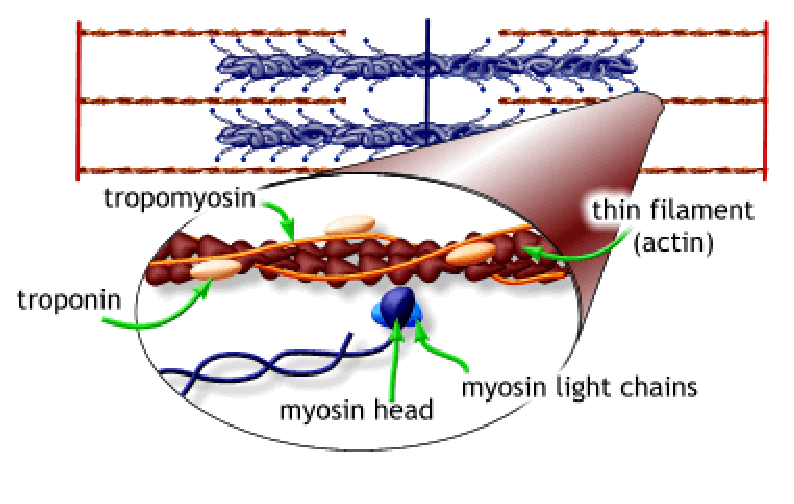
\includegraphics[height=5.5cm]{./images/crossbridge.eps}}
  \caption{A closer look at a sarcomere}\label{fig:crossbridge}
\end{figure}


\subsection{Crossbridge cycle}
\label{sec:crossbridge-cycle}


The crossbridges between the myosins and actins are formed only when
the tropomyosin move out of the way so that myosin heads can reach the
actin, through a process called
{\bf crossbridge cycle}~\cite{chin2006msm}. This is an active process
as it requires ATP\footnote{\url{http://muscle.ucsd.edu/musintro/bridge.shtml}}:
\begin{enumerate}
\item In resting fibre: myosin head (crossbridge) not attach to actin
  (no contraction)

\item When the cell is stimulated to contract, the concentration of
  \ce{Ca^2+} in intracellular environment is increased after the CICR
  process. Some of these \ce{Ca^2+} binds to the protein troponin, and
  causes conformational change that move tropomyosin out of the way,
  leaving spaces for myosin to bind to the actin.\footnote{troponin in
    skeletal myocyte has 4 Calcium-binding sites, while cardiac
    myocyte has 3 Calcium-binding sites}
\item A myosin's head has 2 binding-sites: one for ATP and one for
  actin. In resting fibre, an ATP molecule always bind to it.  As soon
  as the myosin heads bind to the actin filament, the ATP molecule
  binding to it is hydrolysed (to release energy/work). 
  \begin{equation}
    \label{eq:131}
    A + M + ATP \xrightarrow{hydrolysis} A + M + ADP + Pi + Force
  \end{equation}
  with A[ctin], M[yosin]. ATP hydrolysis release ADP, Pi and
  force. The hydorlysis is a force-generating step ( powerstroke) that
  cause the conformation change in the myosin's head (contraction).
\begin{figure}[hbt]
 \centerline{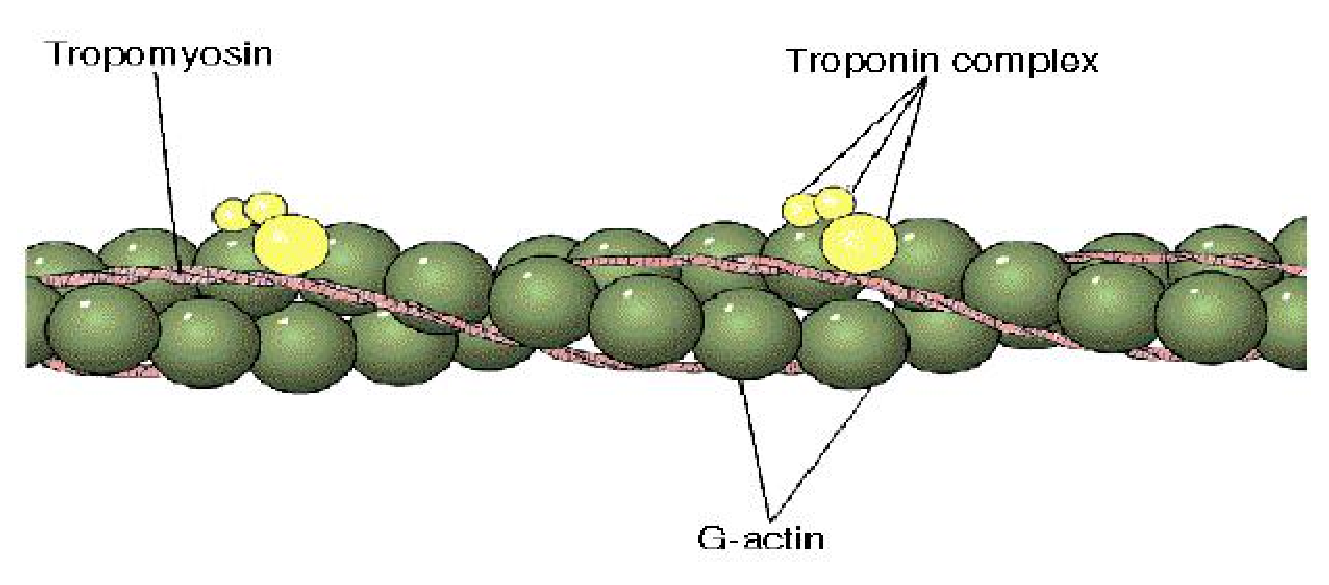
\includegraphics[height=4.7cm,
   angle=0]{./images/thin_filament.eps}}
 \centerline{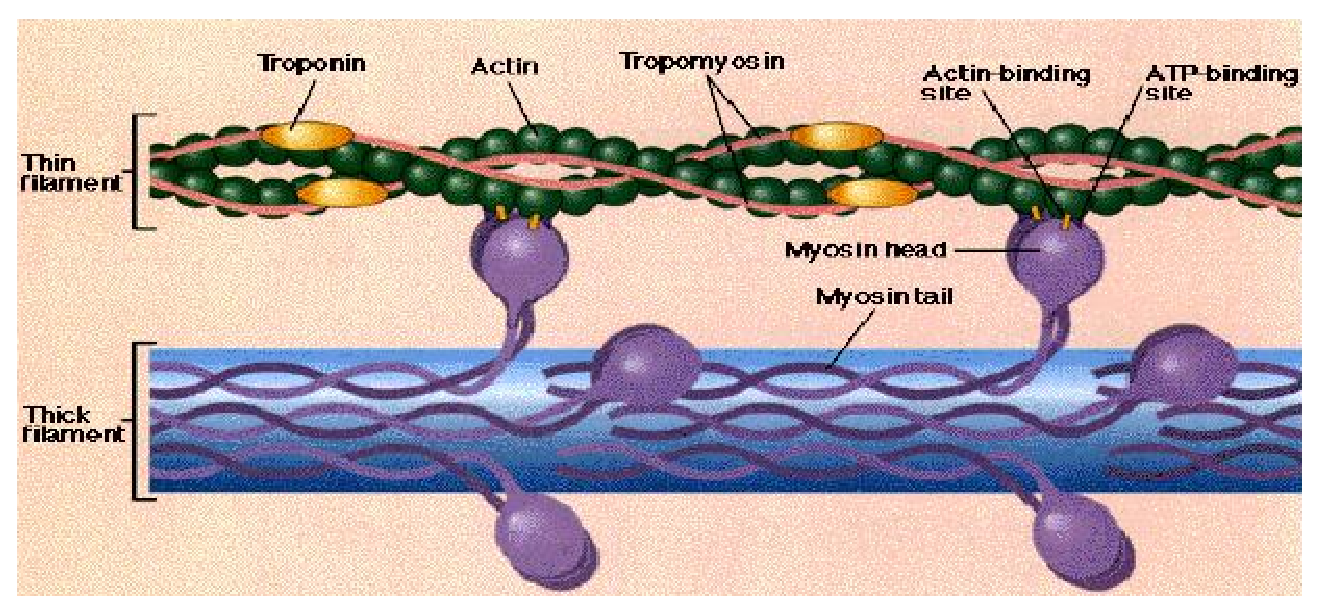
\includegraphics[height=5cm,
   angle=0]{./images/thick_filament.eps}
}
\caption{(A)Thin filament structure (actin), (B) Thick filament (myosin)}
\label{fig:actin_myosin}
\end{figure}

\item After the contraction, another ATP molecule rapidly binds again to the
  myosin's head. The myosin's head turn to it's original shape (relaxation)

\item When the action potential leaves, the \ce{Ca^2+} is retrieved
  and as a result, tropomyosin turns back its conformation, repelling
  the myosin's head from the actin.
\end{enumerate}
This clever mechanism helps the muscle to contract when stimulated by
an electrical impulse\footnote{\url{http://blobs.org/science/article.php?article=38}}. 



\subsection{T-tubule}
\label{sec:t-tubule}

{\bf T-tubule}, known as the transverse tubular system, refers to the
deep invagination of the sarcolemma which facilitates the quick
penetration of the depolarization to the center of the cell. 

In skeletal muscle cells, the T-tubules are typically located at the
junction overlapped between the A-band and I-band. 
T-tubule form 
\begin{enumerate}
  \item triad with the ER membrane in skeletal cell (Sect.\ref{sec:triad})
  
  \item dyad with the ER membrane in cardiac cell (Sect.\ref{sec:dyad})
\end{enumerate}



\section{Cardiac muscles}
\label{sec:cardiac-muscles}

\textcolor{red}{It's important to memorize that both cardiac muscles and
skeletal cells share almost the same structures}. However,
{\it each cardiac muscle cell (as well as a smooth muscle cell) has a
single nucleus, while a skeletal striated cell have multiple nucleus}.
  
Due to the similar structure with skeletal muscle, you are recommended to read
Sec.~\ref{sec:skeletal-muscles} first.
\begin{figure}[hbt]
 \centerline{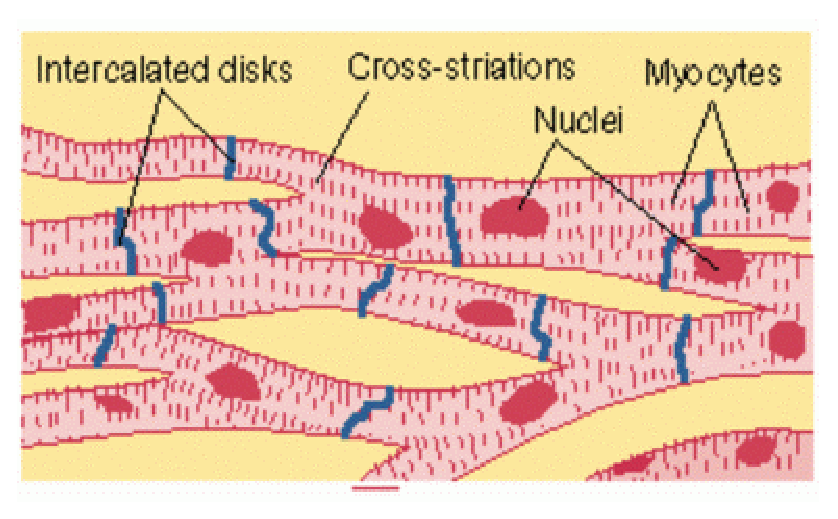
\includegraphics[height=5cm]{./images/cardiac_muscle.eps}}
\caption{Cardiac muscle}
\label{fig:cardiac_muscle}
\end{figure}

Cardiac muscles (cardiac cells) are myocytes {\it found in the heart} and are
extensively tied to one another.  \textcolor{blue}{Before continue reading this
section, reader are recommended to check Chapter 1 of the Cardiology textbook to
learn more about the heart.}


Electron microscopy has advanced our knowledge of the structure and
function of cardiac muscle significantly.  Each small (about $15\times 80\mu m$
on the average) muscle cell is surrounded by a {\it plasmalemma} of unit
membrane configuration. The adjacent myocardial cells are tightly adhered via a
complexes called {\bf intercalated disc} (fascia adherens, desmosome, gap
junction) in which the electrical connection between two neighboring cardiac
cells is conducted via gap junction ({\bf nexus})\footnote{skeletal muscle has
no nexus}, as shown in Fig.~\ref{fig:cardiac_muscle}.


Thus, the heart is not an anatomical {\it syncytium} (i.e. a large cell-like
structure forming by joining two or more cells as a mass of cytoplasm containing
several nuclei but no internal cell boundaries, similar to the structure of
muscle fibers). However, physiologically, the heart act like a syncytium, i.e. a
stimulus given one cell can spread to the whole heart~\cite{sommer1978uhm}. 
Thus, there must be a low resistance pathway between cells, and the underlying
assumptions for modelling the whole-heart using continuum models
(Sect.\ref{sec:continuous-models}).



Around each cell is a plasma membrane known as {\it sarcolemma}.
Cardiac muscles are responsible for the contraction of the heart,
pumping blood to every part of the body.  Thus, cardiac muscles is
highly resistance to fatigue, i.e. it can work for the whole life span
of a human being. In terms of structure, cardiac muscles is similar to
the skeletal muscles.

The primary cell types in the heart are nodal cells
(at SA node and VA node), Purkinje fiber cells, and myocardial cells.
\begin{enumerate}
\item SA nodal cells provide a natural pacemaker signal for the rest
  of the heart. Electrical impulse from the nervous system is
  transmitted to the heart via the junctions with these cells.

\item AV nodal cells is the single gate for the electrical signals
  from the atria to propagate to the ventricles, with a delay.

\begin{mdframed}

There is a group of cells within the heart (at the SA node or VA node)
known as the {\bf pacemaker} or {\bf nodal cells}.
The pacemaker refers to the cell mass that stimulates the heart's
actions. The pacemaker is only responsible for the actual beating of
the heart, not the heart rate. The heart rate is stimulated and
regulated via autonomic innervation. Spontaneous depolarization can
not be handled by the
pacemaker\footnote{\url{http://www.medical-look.com/human_anatomy/organs/Cardiac_muscle.html}}.

\end{mdframed}
 
\item Purkinje fibres cells are primarily for fast conduction.

\item Myocardial cells (both atria and ventricles) are excitable
  muscle cells.
\end{enumerate}
Each time the heart beats, the current flow through the ionic channels in the
plasma membrane cause a characteristic changes in the membrane potential known
as {\bf action potential} (AP) - Sect.\ref{sec:AP-cardiac}.

In cardiac myocytes, calcium play essential role to regulating
excitation-contraction (EC) - Chap.\ref{chap:calc-handl-card}. While the
extracellular sources of calcium remains constant, there is a high variable in
intracellular concentration. In other words, it is the calcium from the
intracellular \ce{Ca^2+} storage that causes the AP. This is described in detail
at Section \ref{sec:cicr}.

\subsection{Atrial cells + Ventricular cells + Conducting cells}

% \section{Cell types: Skeletal vs. Atrial vs. Ventricular myocyte cell
% ultrastructures}

In heart, there are 3 main types of cells:
\begin{enumerate}
  \item Atrial cells: contract in much the same way as skeletal muscle, except
  the duration of contraction is longer
  \item Ventricular cells: contract in much the same way as skeletal muscle, except
  the duration of contraction is longer
  \item Excitatory/conducting cells: these fibers (cells) has the capacity of
  self-excitation (autonomous excitation or autorhtmicity of the heart). They
  are mainly composed of cells in Sino-Atrial (SA) node, Atrio-Ventricular (AV)
  node and Purkinje fibers. 
  
  In human, the SA node fibers discharge at a rate 70/80 bpm; then AV node at
  40-60 bpm; and Purkinje fiber at 14/40 bpm. As SA node has the fastest rate,
  it's the one that set the pace for the rest of the heart. So, SA node is known
  as the pacemaker. 
  
\end{enumerate}


As calcium play an important role to ECC, calcium dynamics is, as a matter of
fact, also discussed too. Due to the major difference of structures between
skeletal muscle and cardiac cells, even thought the ECC processes are similar,
the mechanisms of triggering calcium release are different as well.  The
mechanism for $\Ca$ release is Voltage-Induced Calcium-Release (VICR) in
skeletal cells, and Calcium-Induced Calcium-Release (CICR) in cardiac cells
(Sect.\ref{sec:VICR_CICR}). Thus, the ECC in skeletal muscle depends mostly on
\ce{Ca^2+} release  from the SR, i.e. the role of influx \ce{Ca^2+} is
insignificant; while the EC coupling in cardiac cells depends on both the
\ce{Ca^2+} influx and SR calcium release. 

The ultrastructure in each cell type is well in agreement with this mechanism
difference.
\begin{enumerate}
  \item  To give rise to a homogeneous transient of calcium, in ventricular
  myocyte, the membrane invaginate deep into the interior, forming the so-called
  {\bf transverse-tubular system} (T-tubule). 
  
  \item Ventricular myocyte has an   extensive T-tubular system
  \citep{cheng1994, wier1995}, while atrial cells lack this extensive T-tubular
  system, e.g. rabbit \citep{carl1995}.
  
  \item T-tubules in skeletal muscle have large capacious terminal cisternae
  (junction SR), and small T-tubule (30-40nm); while cardiac cell has a more
  sparse and less rigidly organized SR system with smaller junctional SR, with
  much larger T-tubule (200 nm). 

   \item To make the diffusion from the extracellular space to the interior easier,
cardiac cell has a smaller diameter ($<$ 20 nm thick), compared to that in
skeletal muscle (up to 200 nm). The smaller size of cardiac cells make diffusion
from the extracellular space and T-tubular matrix to the interior of the cells
more plausible. 

The T-tubule invagination forms a complex networks with the sarcoplasmic
reticulum (SR) at the Z-planes. This allows a more uniform influx of $\Ca$ at
all places inside of the cell.
The higher fraction of sarcolemma involved in SR junctions indicate high SR
\ce{Ca^2+}-dependent, e.g. rat (with 6.5-7.7\% in surface and 40-48\% in
T-tubule) is more SR \ce{Ca^2+}-dependent than rabbit (with 4.6\% in surface and
20.6\% in T-tubule), which is more SR \ce{Ca^2+}-dependent than frog (junctional
coupling are very sparse).
   
   \item In ventricular cardiac cells, \ce{Ca^2+} channels is 9 times
higher in concentration in T-tubules than in the external  sarcolemma. It
particularly localized over junctional SR containing RyR. This is known as
calcium release units (sites) (CRUs). So, the $\Ca$ transient is often uniformly
in the cells, while that in skeletal cells, the $\Ca$ waves start from the outer
membrane then propagate to the inner of the cell (Chapter
\ref{chap:calcium_waves_RYR}).
       
\end{enumerate}

\begin{figure}[hbt]
  \centerline{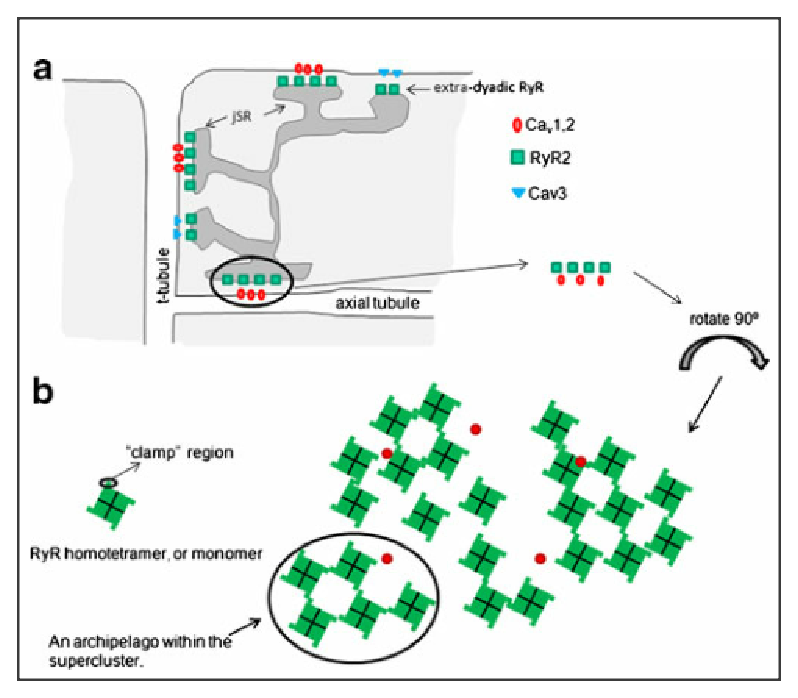
\includegraphics[height=7cm,
    angle=0]{./images/couplon_axial.eps}}
\caption{Couplons are formed on both the plasmalemma, T-tubules and axial
tubules \citep{asghari2009}}
\label{fig:couplon_axials}
\end{figure}

It's well known that T-tubules is a common feature in cardiac ventricular
myocytes. However, recent experimental data shown that it's also a common
feature in atrial cells of large mammals (sheep), including human
\citep{kirk2003, richards2011}. In atrial cell, many do possess an irregular
internal transver-axial tubular system (TATS) \citep{kirk2003}, with axial tubules
branching from T-tubules, Fig.\ref{fig:couplon_axials}. However, the proportion
of  axial junctions, their sizes, and the number of RyR2s on axial tubules are
unknown. Not until recently, some studies have shed a light into the role and
structures of axial tubules
\citep{asghari2009}. For more detail, read Sect.\ref{sec:t-tubular_system}


% \begin{figure}[htb]
%   \centerline{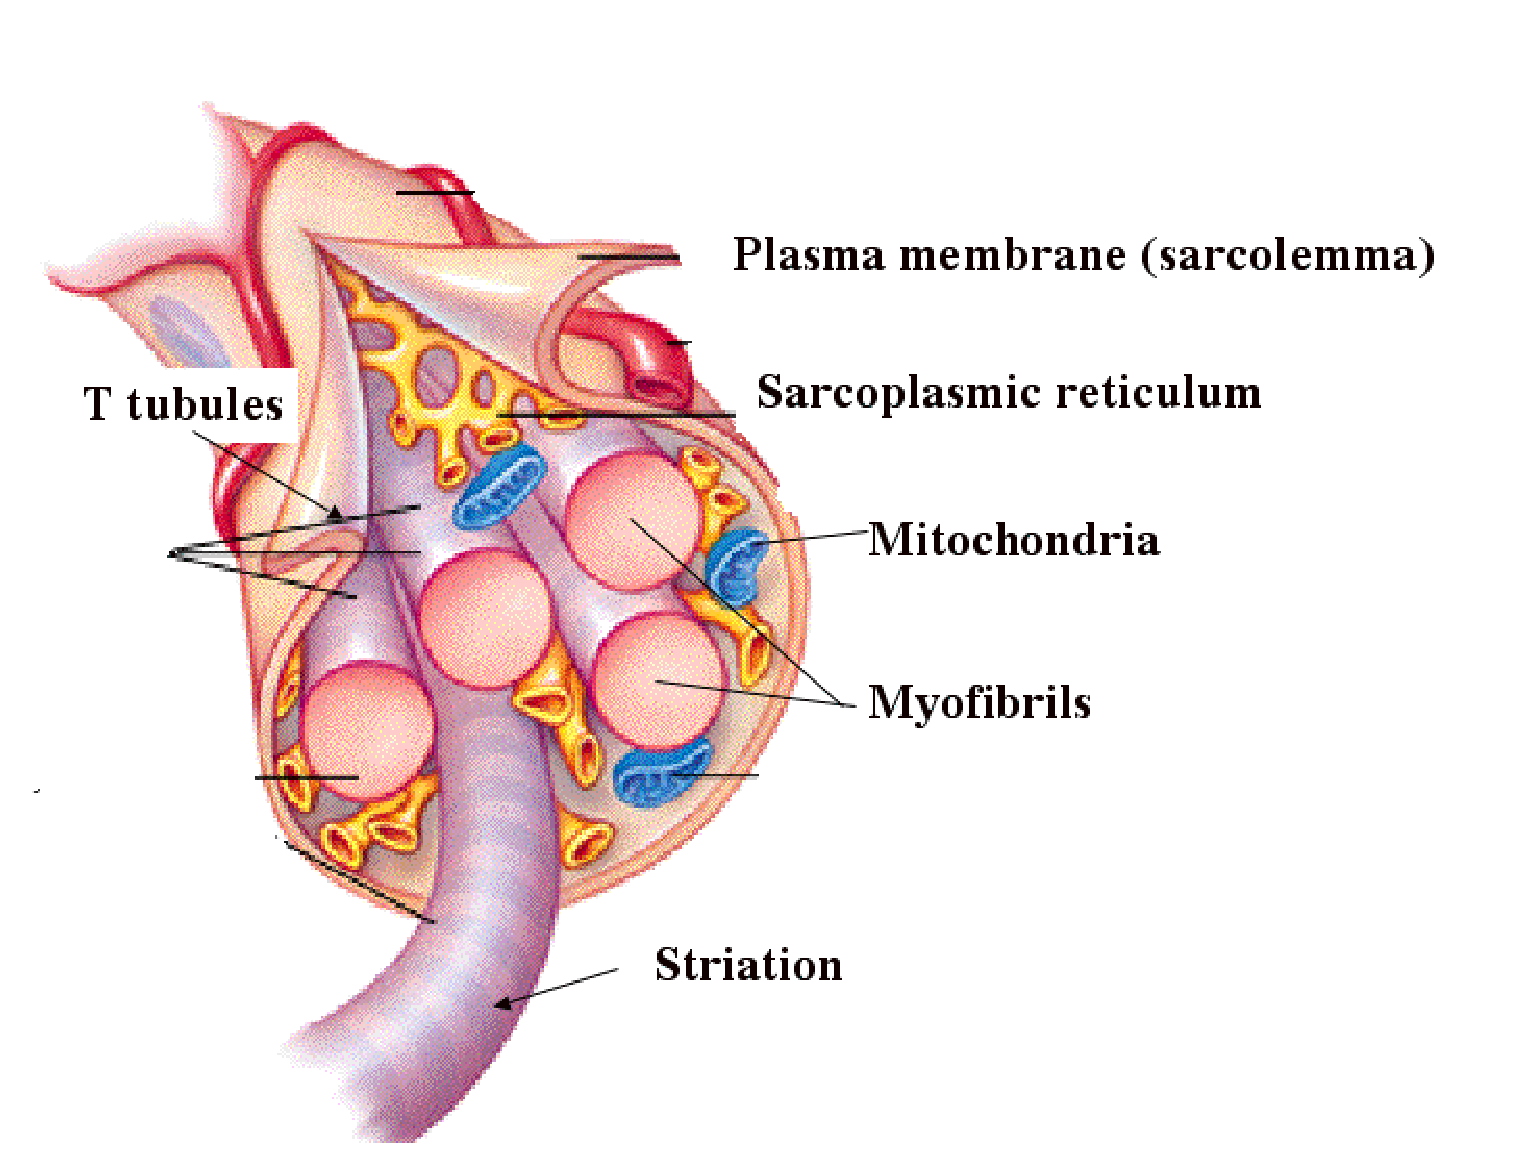
\includegraphics[height=7cm]{./images/MuscleCell.eps}}
%   \caption{Muscle cells}\label{fig:muscle_cell}
% \end{figure}

\subsection{T-tubular system}
\label{sec:t-tubular_system}

The sarcotubular system in mammalian ventricular heart muscle cells was first
identified using electron microscopy (EM) \citep{lindner1956}. The data showed
that tubular system was continuous with the sarcolemma, invaginated deep into
the inner side of the cell and located at the level of the Z-lines
\citep{girardier1964}.
They were assumed to run traversely and hence were named {\bf transverse tubular
system} (T-tubular system). As the T-tubule is continuous with the sarcolemma,
along with the cell membrane, they are collectively called ``the sarcolemma''.
If we means to exclude the T-tubule, we can call surface sarcolemma (external
sarcolemma). A large (T-tubule volume):(T-tubule surface area) ratio in cardiac
T-tubules means that there is small depletions and accumulation of $\Ca$ ions in
the T-tubules during the cellular activity. This allows us to treat the
sarcolemmal as invading into every inner place in the cell.

T-tubules are found in the cardiac tissues of all species of mammals so far
investigated (e.g. rats, mice, guinea pigs, rabbits, dogs, pigs, and humans),
but appear to be absent in avian, reptile, and amphibian cardiac tissue
\citep{brette2003}. Within mammalian cardiac tissues, T-tubules are far less
developed in atrial, pacemaking, and conducting tissue. Recent reports
suggested that about 50\% of atrial myocytes possess a sparse irregular
T-tubular system \citep{kirk2003, richards2011}.


Subsequent studies shown that a considerable amount of tubules run in the axial
directions \citep{forssmann1970, sperelakis1971}.
Later on, a better descriptive name was given to it ``transverse-axial tubular
system'' (TATS or T-Ax) \citep{forbes1984, amsellem1995}. However, there are
also large numbers of tubules that run neither axial nor transverse directions.
It's thus suggested to use the term ``Sarcolemma Z rete'' (SZR)
\citep{soeller1999}. EM suggests that tubules have nearly circular
cross-sections, with the majority of tubules appear in diameters of 200-300nm,
Fig.\ref{fig:T-tubules_diameter}. Most tubules (51\%) are between 180 and 280nm
wide \citep{soeller1999}. No tubules largers than 450nm were found.

\begin{figure}[hbt]
  \centerline{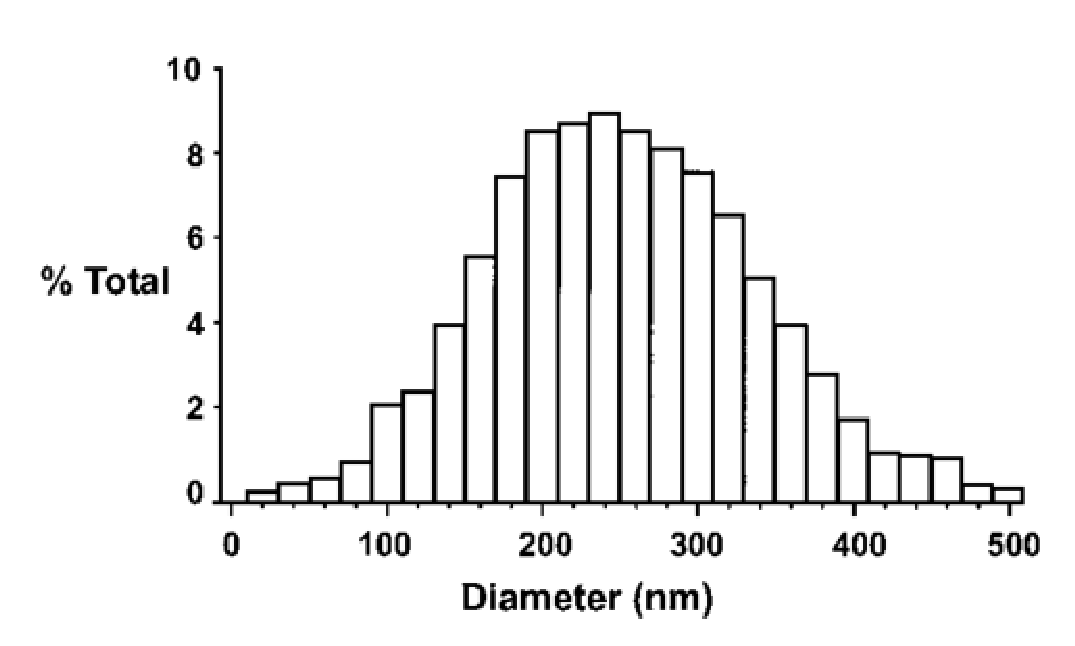
\includegraphics[height=4cm,
    angle=0]{./images/T-tubule_diameter.eps}}
\caption{Distribution of T-tubules diameter \citep{soeller1999}}
\label{fig:T-tubules_diameter}
\end{figure}



\begin{framed}
The drawback of EM method is that the specimen must be fixed (or frozen),
dehydrated, thin sectioned and heavy-metal stained. The ``thick EM sections''
are limited to about 5$\mum$ \citep{peachey1986}, while a cell thickness is
about 10$\mum$. Thus, typically, only a section of 11x24x2-$\mum$ section of the
TATS in a mouse myocardial is shown using EM. Also, the image has no intrinsic
3D-resolution, so the 3D reconstruction of T-tubules orientation from stacks of
thin EM sections images is very complicated. Using manual section registration,
only a 5.5$\mum$-thick segment of a heart cell can be reconstructed
\citep{amsellem1995}.
\end{framed}

By immersing the cells with a soluble fluorescent marker that penetrate the
tubular system but not cross the cell membrane (i.e. dextran-linked
fluorescein), \citep{soeller1999} used 2-photon molecular excitation (TPME)
microscopy to detect the 3D structure of T-tubule system. \citep{kirk2003} used
Di-8-ANEPPS to label TATS in cardiac atrial cells. The binary image representing
the location of T-tubular systems was created (intensities greater than the mean
background + 5 SD were assumed to represent t-tubular segments and get values
1.0; otherwise, use 0.0). The tubule signal intensity was removed and replaced
with a thin line of uniform thickness, representing the T-tubular system. NOTE:
Tubules less than 50nm in diameter may be lost in the noise. Since the smallest
t-tubule diameter reported in left ventricular myocytes of rat is about 70nm,
the limit were considered acceptable \citep{soeller1999}.



Some evidences have suggested that T-tubules system may not be a fixed
structure. In particular, short-term cell culture has been reported to be
associated with a loss of T-tubules \citep{lipp1996snu}, and T-tubule
proliferation occurs with hypertrophy \citep{page1973}. 


The loss in T-tubules also exhibit marked spatial inhomogeneities in calcium
transient in guinea-pig ventricular myocytes \citep{lipp1996snu}. 

\section{Cardiac muscle data}
\label{sec:cardiac-muscle-data}

\subsection{Capacitance}
\label{sec:capacitance-cardiac-muscle}


Capacitance (Sect.\ref{sec:capacitance}) of rat ventricular myocyte, measured
from the integral of the current transient resulting from +5mV depolarizing
voltage-step
\begin{enumerate}
  \item (rat) 99$\pm$8 pF with cell volume 16 pL (100x21x7
  $\mum^3$) or the capacitance-to-volume ratio is
  6.2$\pm$0.5 pF/pL \citep{Bouchard1995}
  
  \item (rat) 
\end{enumerate}


\subsection{Membrane surface area ($A_m$)}
\label{sec:surface_area_membrane}

Based on the fact that one centimeter square of cell membrane has about 1$\muF$
capacitance (Sect.\ref{sec:specific-membrane-capacitance}), measuring the cell
capacitance is a good indicator of surface membrane area of cells. There's a
positive linear correlation between membrane capacitance Acap ($\muF$) and cell
surface area Am ($\cm^2$) in each animal species.
\begin{verbatim}
Acap = Am * Cm          ! [uF]
\end{verbatim}
with $\Csc=1\mu$F/cm$^2$, i.e. Acap is calculated from 5 mV clamp for 20ms,
applied for holding potential -80mV.

% The membrane surface area is often derived from the measured capacitance given
% the fact that specific capacitance is $\Csc = 1\muF/cm^2$.
The capacitance is also an indirect index for estimating cell volume. However,
using optical microscopy, \citep{satoh1996svr, delbridge1997} has proposed that
surface area-to-cell volume-ratio is pretty constant
(Sect.\ref{sec:volume-surf-relat})

\begin{mdframed}
If patch is used, the dimension of a nucleated patch can be measured by DIC
infrared microscopy, and then can be approximated by assuming the ellipsoid
shape. The surface area is \citep{gentet2008}
\begin{verbatim}
surface area = (major axis + minor axis)^2 * (pi/4)
\end{verbatim}

\end{mdframed}

Other measurement: \citep{gentet2008} for \textcolor{red}{HEK-293 cells} whose
dimensions were measured using phase-contrast microscopy; and the measurement
was done twice: first assumed a smooth ellipsoid, then measured again once the
cells were expanded in response to internal pressure. Pressure was applied in an
attempt to flatten out the filopodia and permit a more accurate estimate of
total membrane surface area under light microscopy.
The perimeter of the cell, including its processes, was estimated using NIH
Image software
\begin{verbatim}
total surface area = perimeter^2 / pi
\end{verbatim}
A few fine processes were lost during the automated image enhancement,
so this approach may slightly underestimate the membrane surface area.



\begin{enumerate}
  \item Sprague-Dawley rat: (control) 8.9$\pm$0.3 pF/pL,
  (pressure-overload hypertrophy) 8.5$\pm$0.4 pF/pL
  
  \item Sprague-Dawley rat (250-300g) (22$^\circ$C):
  6.1$\pm$0.5 pF/pL (cell dimension: 110x21x7 $\mum^3$ and
  cell volume 16pL) \citep{Bouchard1995}
\end{enumerate}

\subsection{Cell Volume (V$_\text{cell}$)}
\label{sec:volume-surf-relat}

The amplitude of ionic currents is dependent not only on the membrane potential,
transarcolemmal ionic gradients, but also on cell size. The exact knowledge of
the cell volume is very important in quantifying the contribution of ion fluxes
through the membrane channels to the changes of intracellular ion
concentrations. 

A stacks of X-Y line-scan images of cellular fluorescences obtained at high
spatial resolution throughout the entire depth of the cell was collected (20-35
sections at 1.2$\mum$ steps depending the cell thickness).
The cell volumes were generated using 3D volume rendering from these images
\citep{satoh1996svr}. An individual pixel was exposed to the laser light for $<
4\mus$, which requiers 1.04sec for an X-Y image. The spatial resolution in axial
direction (z-dimension) was estimated to be $<1\mum$, so the sectioning interval
was chosen of 1.2$\mum$ to avoid out-of-focus contributions. A binary threshold
was chosen to set pixels belonging to the cell and pixel fall into the
extracellular regions. However, photobleaching may affect to pixel intensities,
care need to be taken to keep photobleaching to a minimum (i.e. using lowest
laser power).

The volumes was calculated as, Table.\ref{tab:volume_data}
\begin{enumerate}
\item rabbit: $30.4\pm 7.3$pL
\item ferrets: $30.9\pm 9.0$pL
\item rats: $34.4\pm 7$pL
\end{enumerate}

\begin{table}[hbt]
\begin{center}
    \begin{tabular}{lccc}
        \hline
        & Rabbit & Ferret & Rat \\
    \hline \hline
    Length ($\mum$) & 142.8$\pm$29.5 & 130.0$pm$22.7 & 141.9$\pm 14.9$ \\
	Width ($\mum$) & 31.9$\pm 9.5$ & 31.0$\pm 5.3$ & 32.0$\pm 4.8$ \\
	Depth ($\mum$) & 12.1$\pm 1.7$ & 14.0$\pm 2.8$ & 13.3$\pm 1.6$\\
	$\Cm$ (pF)  &   138.0$\pm 31.3$ & 162.4$\pm 35.6$ & 289.2$\pm 68.8$ \\
    \end{tabular}
\end{center}
\caption{Data in rabbit, ferret and rat ventricular myocytes \citep{satoh1996svr}}
\label{tab:volume_data}
\end{table}

The cell morphology at different stage of lifes for rat ventricular myocytes is
given in Table.\ref{tab:volume_data_rat_young_adult}.

\begin{table}[hbt]
\begin{center}
    \begin{tabular}{lcc}
        \hline
        & Adolescence & Adult \\
    \hline \hline
    Length ($\mum$) & 123.8$\pm$14.4 &  140.1$\pm 16.4$ \\
	Width ($\mum$) & 33.6$\pm 6.7$ & 33.4$\pm 4.8$ \\
	Depth ($\mum$) & 12.8$\pm 1.4$ & 13.8$\pm 1.5$\\
	Volume (pL) & 30.9$\pm 5.2$ & 36.8$\pm 6.3$ \\
	$\Cm$ (pF)  &   207.2$\pm 30.5$ & 323.9$\pm 51.8$ \\
    \end{tabular}
\end{center}
\caption{Data in rabbit, ferret and rat ventricular myocytes \citep{satoh1996svr}}
\label{tab:volume_data_rat_young_adult}
\end{table}

Assuming the cell with a simple geometry of rectangular parallelepiped
(length*width*depth), the rendered volume values are 54\% of the volume of the
parallelpiped. Assuming the cell with a spindle-shaped cell geometry, then the
estimated volume is 42\% larger than the calculated volume. Assuming the cell
with a rod-shaped geometry with an ellipsoidal cross-section, then the estimated
volume is 29\% smaller than it \citep{satoh1996svr}.

\subsection{* In relation with external cell surface and cell diameter}

Using the detected surface membrane area, the question is can we estimate  cell
volumes? This is not easy due to (1) the different degree of membrane folding
and the abundance of membrane invagination in different cell types, (2)
development stages. ~\citep{satoh1996svr} first carried out a study to see how
cell surface (external sarcolemma) related to cell volumes. 
The ratio of (cell external sarcolemma area)/(cell volume) is an
inversely related to cell diameter. 

If we assume the cell has cylindrical shape of radius \verb!radius!,
then
\begin{verbatim}
(cell external sarcolemma area)/(cell volume) = 2/radius
\end{verbatim}

\subsection{* In relation with cell capacitance}

The cell volume (pL) is expressed in the form of cell capacitance (pF), i.e.
pF/pL (Sect.\ref{sec:capacitance-cardiac-muscle}). 

Despite the large variability in the cell sizes, the capacitance-volume ratio
$\Acap/V_\cell$ or $\Cm/V_\cell$ was quite constant and is measured as,
Table.\ref{tab:volume_data}.
\begin{enumerate}
\item rabbit: $4.58\pm0.45$ pF/pL
\item ferret: $5.39\pm 0.57$ pF/pL
\item rats: $8.44\pm 1.35$ pF/pL
\end{enumerate}

At different developmental stage, this ratio varies for a single
species as well, e.g. in 6-month-old rat it is $8.88\pm1.14$pF/pL, and
in 3-month-old rat is $6.76\pm0.62$ pF/pL.

\begin{enumerate}
\item rabbit:
  \begin{equation}
    \label{eq:1436}
    V_\cell = 0.215*\Cm + 0.718
  \end{equation}
\item ferret:
  \begin{equation}
    \label{eq:1437}
    V_\cell = 0.192*\Cm + 0.07
  \end{equation}
\item rat:
  \begin{equation}
    \label{eq:1438}
    V_\cell = 0.078*\Cm + 11.755
  \end{equation}
\end{enumerate}


\subsection{* In relation with cell length, width}

Cell length and width are easy to measure parameters using conventional light
microscopy (without using confocal microcopy). Then, cell length and width can
be used to extrapolate cell volume too, using the linear correlation, the cell
volume (in pL) is given as
\begin{enumerate}
\item rabbit:
\begin{equation}
  \label{eq:1439}
  V_\cell = 6.59\times 10^{-3} (\text{pL/cm}^2) \times \text{cell area} (\mu\text{m}^2)
\end{equation}
\item ferret:
\begin{equation}
  \label{eq:1440}
  V_\cell = 7.21\times 10^{-3} (\text{pL/cm}^2) \times \text{cell area} (\mu\text{m}^2)
\end{equation}
\item rat:
\begin{equation}
  \label{eq:1441}
  V_\cell = 7.59\times 10^{-3} (\text{pL/cm}^2) \times \text{cell area} (\mu\text{m}^2)
\end{equation}
\end{enumerate}

\subsection{Volume fractions}
\label{sec:volume-fractions}

Peachey (1965) reported the skeletal muscle T-tubular area is $\sim$ 7 times the
area of external sarcolemma. In mammalian, 30-5\% the area of the sarcolemma is
in the T-tubules, and in mammalian atrium, this fraction is $<$ 15\%. Soeller \&
Cannell (1999) detected 64\% of sarcolemma in T-tubule, and 60\% of the
T-tubular area is within 0.55 $\mu$m of the Z-line.

%  However, it's
% important to know that a large fraction of the cell volume is occupied
% by the myofilament and the mitochondria; the effective cell volume is
% $V_{cyto} = 10$pl $< V_\text{cell}$. 


Among cell volume:
\begin{enumerate}
\item T-tubules occupy 3.6\% of the cell volume \citep{soeller1999} in rat
(earlier estimation using EM showed 1\% in rat \citep{page1973}) with estimated
surface area of t-tubule membrane per unit cell volume is 0.44$\mum^2/\mum^3$
(about three times larger than previously reported stereological measurements
using EM of 0.15$\mum^2/\mum^3$).

\item SR volume: 3.5\% of rat cell volume \citep{page1971, page1978}

\item Mitochondria: 20-36\% of cell volume

Mitochondria occupy 35\% (rat), 32.2\% (ferret),  38.9\% (rabbit) of the cell
volume \citep{barth1992}
 
\item Myoplasm occupy 65\% (atrial cell), 50\% (ventricle)

\item Myofilament occupy 45-60\% of the cell volume
\end{enumerate}
The sarcoplasmic reticulum (SR) extends throughout the entire cytoplasm, yet
only occupies 4\% of the ``cytoplasmic'' volume in rabbit ventricular myocytes. 
NOTE: surface to volume rate (in pF/pL) and electrophysiological measurement of
ion flux (in pA/pF or pmol/pF) can  be translated into fluxes per unit cell
volume ($\mu$M).


In terms of surface area of sarcolemma vs. T-tubule:
\begin{enumerate}
  \item Rat ventricle: T-tubular area is 21-33\% of sarcolemma
  \item Frog skeletal: T-tubular area is $\sim 7$ times the area of external
  sarcolemma
  \item Mammalian skeletal: somewhat less dominant (compared to that of frog
  skeletal), but still relatively large.
  \item Mammalian ventricle: T-tubule area is 30-50\% of SL area.
  \item Mammalian atrium: T-tubule area is $< 15\%$ of SL area. Some reports
  shown no T-tubule in mammalian atrium, or $\sim 20$ times less T-tubular area
  in rabbit atrium vs. ventricle. 
  \item Many species lack T-tubule: bird, amphibian, reptilian hearts.
\end{enumerate}
The cell diameters also affect to the (external sarcolemma area)/(cell volume)
ratio (See Sect.\ref{sec:volume-surf-relat}). It means smaller cells have higher
(surface/volume) ratio, and T-tubules are less important for $\Ca$ activation
and diffusion than in mammalian cells or cells with larger diameter. 

The spatial distribution of ion channels is important in spatial models:
\begin{enumerate}
  \item Skeletal muscle: density of $\Na$ channels, delayed rectifier K
  channels, and Na/K-ATPase pump is lower in skeletal muscle T-tubules than on
  surface sarcolemma; while density of $\Ca$ channels is $> 4$ times higher in
  T-tubules (Bers' book, page 2).
  
  \item Rat: 21-33\% of sarcolemma being T-tubule, and 75\% of LCCs are in
  T-tubules. So, the density of LCC in T-tubule is $\sim 9$ times higher than
  that in external sarcolemma. 
  
  \item Rabbit ventricule: LCC is colocalized with RyR and triadin at dyads in
  T-tubules
  
  \item Rabbit atrium and ventricle: DHPR mainly on surface sarcolemma and is
  localized with junctional SR containing peripheral RyRs, i.e. all dyads are
  peripheral. This is similar to chicken heart.
\end{enumerate}



The SR is a sac-like structure which forms a dense network of
interconnected T-tubules and cisternae. The cisternae is often
referred to as {\it junctional SR} (JSR); and the SR tubular network
is called {\it network SR} (NSR). These cisternae are localized in
closed proximity to the T-tubules. The space between the cisternae and
the T-tubule is called the {\bf dyadic subspace} or
{\it dyadic junction} (NOTE: dyadic or dyadic the same). Average
volume of a dyadic subspace is $\sim 10^{-9}$ times of the cell
volume. The site where SR comes into closed intact with sarcolemma is (1) almost
exclusively in T-tubules (skeletal muscle); (2) mostly in T-tubules in mammalian
ventricles or, (3) primarily on the surface sarcolemma (mammalian atrium and
avian heart). 





\subsection{Rat ventricle}

Based on the cell volume of 36 pL (rat ventricle 6 month). 
\begin{enumerate}
  \item Nucleus is 2\%, i.e. volume is 0.72 (pL). However, in modeling we ignore
  nucleus, and assuming this becoming myoplasm
  \item Myoplasm is 48\%, becoming 50\% with nucleus included, i.e. volume is 18
  (pL)
  \item T-tubule is 1.2\%, i.e. 0.432 (pL)
  \item SR is a reticular, luminally continuous compartment, occupying 3-4\% of
  cell volume \citep{page1978,brochet2005}. We used SR total is 3.5\%, i.e. 1.26
  (pL).
  With NSR is 3.2\%, i.e.
  1.152 (pL) and JSR is 0.3\%, i.e. 0.108 (pL). 
  \item The total SR surface area is 42.5\% of cell volume, i.e. 1.53d-4
  (cm$^2$). Here, external SR is 0.24 and T-tubule is 0.44 which is 0.68
\end{enumerate}

\citep{soeller1999} shown that in rat ventricle
\begin{itemize}
  \item T-tubules occupy 3.6\% of cell volume, (sarcolemma surface area)/(cell
  volume) is 0.44 ($\mum^2/\mum^3$); and 64\% of sarcolemma is T-tubules, i.e. (external
  sarcolemma)/(cell volume) is 0.24$\mum^2/\mum^3$. 
  
\end{itemize}



\section{3D visualization/reconstruction of the data}

A flexible and powerful 3D visualization is IrisExplorer by NAG.



%%% Local Variables: 
%%% mode: latex
%%% TeX-master: "thermo-stat"
%%% End: 
